\subsection{Signal extraction}\label{sec:WBoson_Analysis_SignalExtraction}

The signal and background event yields are extracted by fitting the \ptmiss distribution from data. The background events correspond to high-\pt muons that satisfy the signal selection criteria and are not produced from a direct decay of a \Wb boson. A brief description of the background sources considered in this analysis is given below:

\begin{itemize}

 \item QCD jet: constitute high-\pt muons produced from semi-leptonic decays of heavy-flavour hadrons formed within jets. Such muons are generally surrounded by a large hadronic activity and their contribution is significantly suppressed by selecting isolated muons ($\iso < 0.15$). However, muons from hadron decays can sometimes pass the isolation criteria and thus, a small fraction of the QCD jet background remains in the signal region.

 \item $\DYToMuMu$: a high-\pt muon produced from a \Z-boson decay or Drell--Yan. The contribution from this process is suppressed by applying the \DYToMuMu veto, which excludes events containing at least one pair of well-identified isolated muons, each with $\pt > 15$~\GeVc. The \DYToMuMu events, in which one of the two muons is produced outside of the CMS coverage ($\abs{\etaLAB}<$ 2.4) or does not satisfy the muon selection criteria, survive the veto. Such events are expected to contribute more in the CMS endcap regions ($|\eta| > 2.0$), where one of the muons from the \DYToMuMu decay escapes the detector producing a large \ptmiss.

 \item $\ttbar\rightarrow\mu\nu_{\mu}+X$: a high-\pt muon from semi-leptonic decays of top (anti-)quarks. The inclusive cross section of top-quark pair production in \pPb at $\sqrtsnn = \SI{8.16}{\TeV}$, has been measured by the CMS collaboration to be $\sigma_{\ttbar} = 45 \pm 8$~nb~\cite{HIN-17-002}. The \ttbar process is expected to have a very small impact in the signal region due its small inclusive cross section and its branching ratio (13.4\%) to muons~\cite{PDG}.

 \item $\WToTauNu \rightarrow\mu\nu_{\mu} + X$: consists of the leptonic decay of a \Wb boson into a \PGt lepton, which then decays into a high-\pt muon.

 \item $\DYToTauTau\rightarrow\mu\nu_{\mu}+X$: corresponds to a ditau decay of a \Z boson or virtual photon, where one of the \PGt leptons then decays into a high-\pt muon.
 
\end{itemize}

The largest source of background in the signal region corresponds to QCD jets which represent approximately 18\% of events in data. Among the electroweak background processes, the dominant one is the \DYToMuMu background. The electroweak background amounts to roughly 12\% of the events in the signal region, divided as: \DYToMuMu ($9\%$), \WToTauNu ($2\%$) and \DYToTauTau ($1\%$). The \ttbar background contributes roughly $0.5\%$ of  events. Other electroweak processes such as double boson decays ($\Wb\Wb$, $\Wb\Z$ and $\Z\Z$) have been checked to contribute less than 0.03\%, so they are not considered.

The shape of the QCD jet background is modelled using a functional form derived from data as explained in \sect{sec:WBoson_Analysis_SignalExtraction_QCDBackground} and the shapes of the signal, \ttbar background and electroweak background are estimated using the \ptmiss distribution from simulations, as described in \sect{sec:WBoson_Analysis_SignalExtraction_EWKBackground}. \sect{sec:WBoson_Analysis_SignalExtraction_FitModel} introduces the model used to extract the signal. The event yields obtained from the fits are presented in \sect{sec:WBoson_Analysis_SignalExtraction_RawYields} and corrected for efficiency in \sect{sec:WBoson_Analysis_SignalExtraction_CorrectedYields}.

\subsubsection{Modelling of the QCD jet background}\label{sec:WBoson_Analysis_SignalExtraction_QCDBackground}

The QCD jet background cannot be simulated reliably in \RunpPb collisions due to the imprecise knowledge of the production cross sections and nuclear modifications of hadrons, and the inaccurate modelling of the event activity. Thus, a data-driven approach is used to determine the \ptmiss distribution of the QCD jet background.

The overall procedure consists of the following steps: first the parametrisation of the QCD jet \ptmiss distribution in a region dominated by non-isolated muons, then the determination of the dependence of the QCD jet \ptmiss functional form with respect to the muon isolation and finally the extrapolation of the  QCD jet \ptmiss functional form to low muon isolation values, namely in the signal region.

The \ptmiss distribution of the QCD jet background is parametrised by a modified Rayleigh distribution, defined as:

\begin{equation}
 f_{\text{QCD}}\left(\ptmiss\right) = \ptmiss{\cdot}\exp\left(-\frac{\left(\ptmiss\right)^{2}}{2\left( \sigma_{0} + \sigma_{1}\cdot\ptmiss + \sigma_{2}\cdot\left( \ptmiss \right)^{2} \right)^{2}} \right)
 \label{eq:QCD_Nominal}
\end{equation}

where $\sigma_{0}$, $\sigma_{1}$, and $\sigma_{2}$ are free parameters extracted by performing an unbinned maximum-likelihood fit to the \ptmiss distribution in a control sample from data. The events in the control sample are selected by applying all signal selection requirements, except the muon isolation cut. The fits are performed separately for positive and negative charged muon events.

To derive the muon isolation dependence of the QCD jet background parameters, the \ptmiss spectrum in the control sample is fitted with the QCD jet \ptmiss functional form, in five bins of the muon isolation variable with the following boundaries: [ 0.4 , 0.5 , 0.6 , 0.7 , 0.8 , 0.9 ]. Lower muon isolation values ($\iso < 0.4$) are discarded, due to the large contamination from weak boson decays. The results of the QCD jet background fits, corresponding to the lowest and highest muon isolation regions, are shown in \fig{fig:QCD_Fits}.

\begin{figure}[htb!]
 \centering
  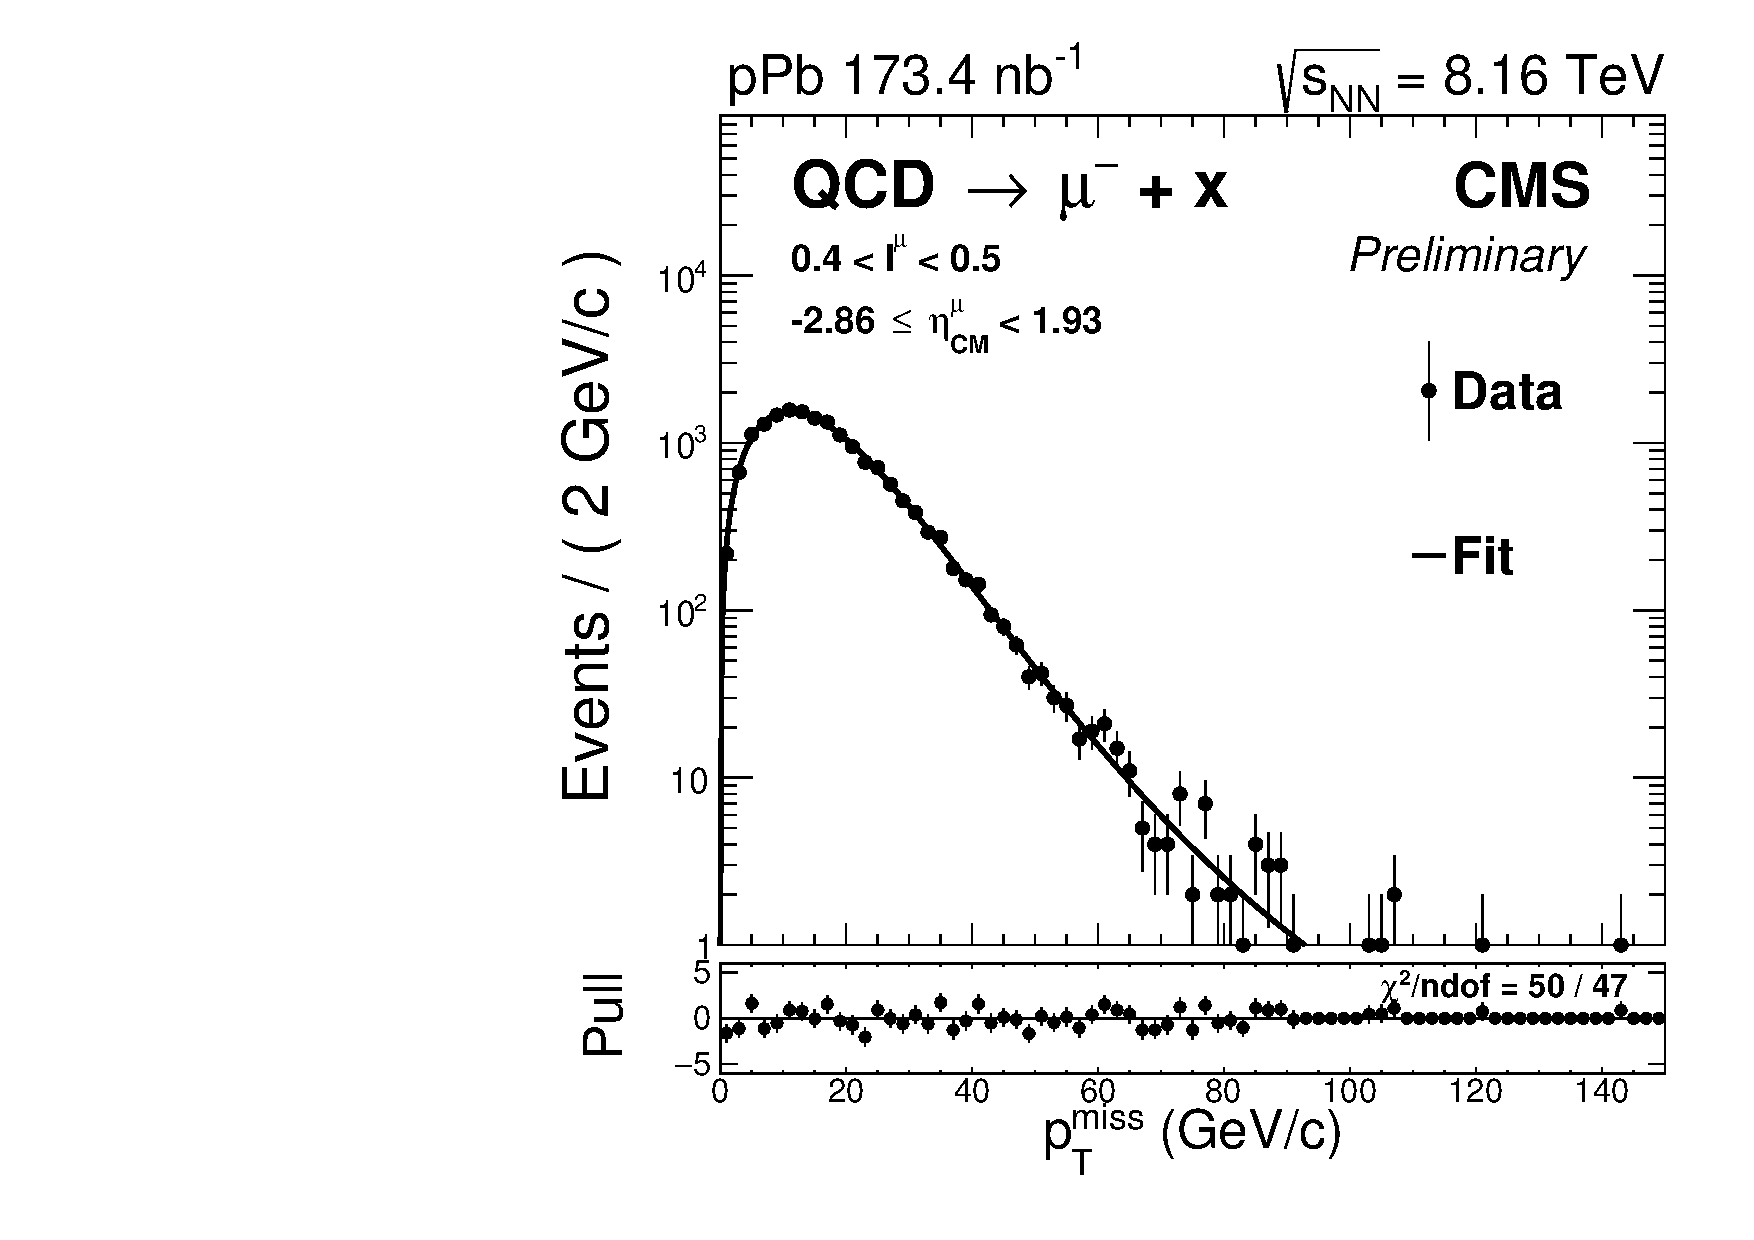
\includegraphics[width=0.45\textwidth]{Figures/WBoson/Analysis/SignalExtraction/QCD_Template/DATA/PLOT_MET_DATA_QCDToMuMi_PA_Model_ModifiedRayleigh_MuEtaCM_-286_193_MuIso_40_50.pdf}
  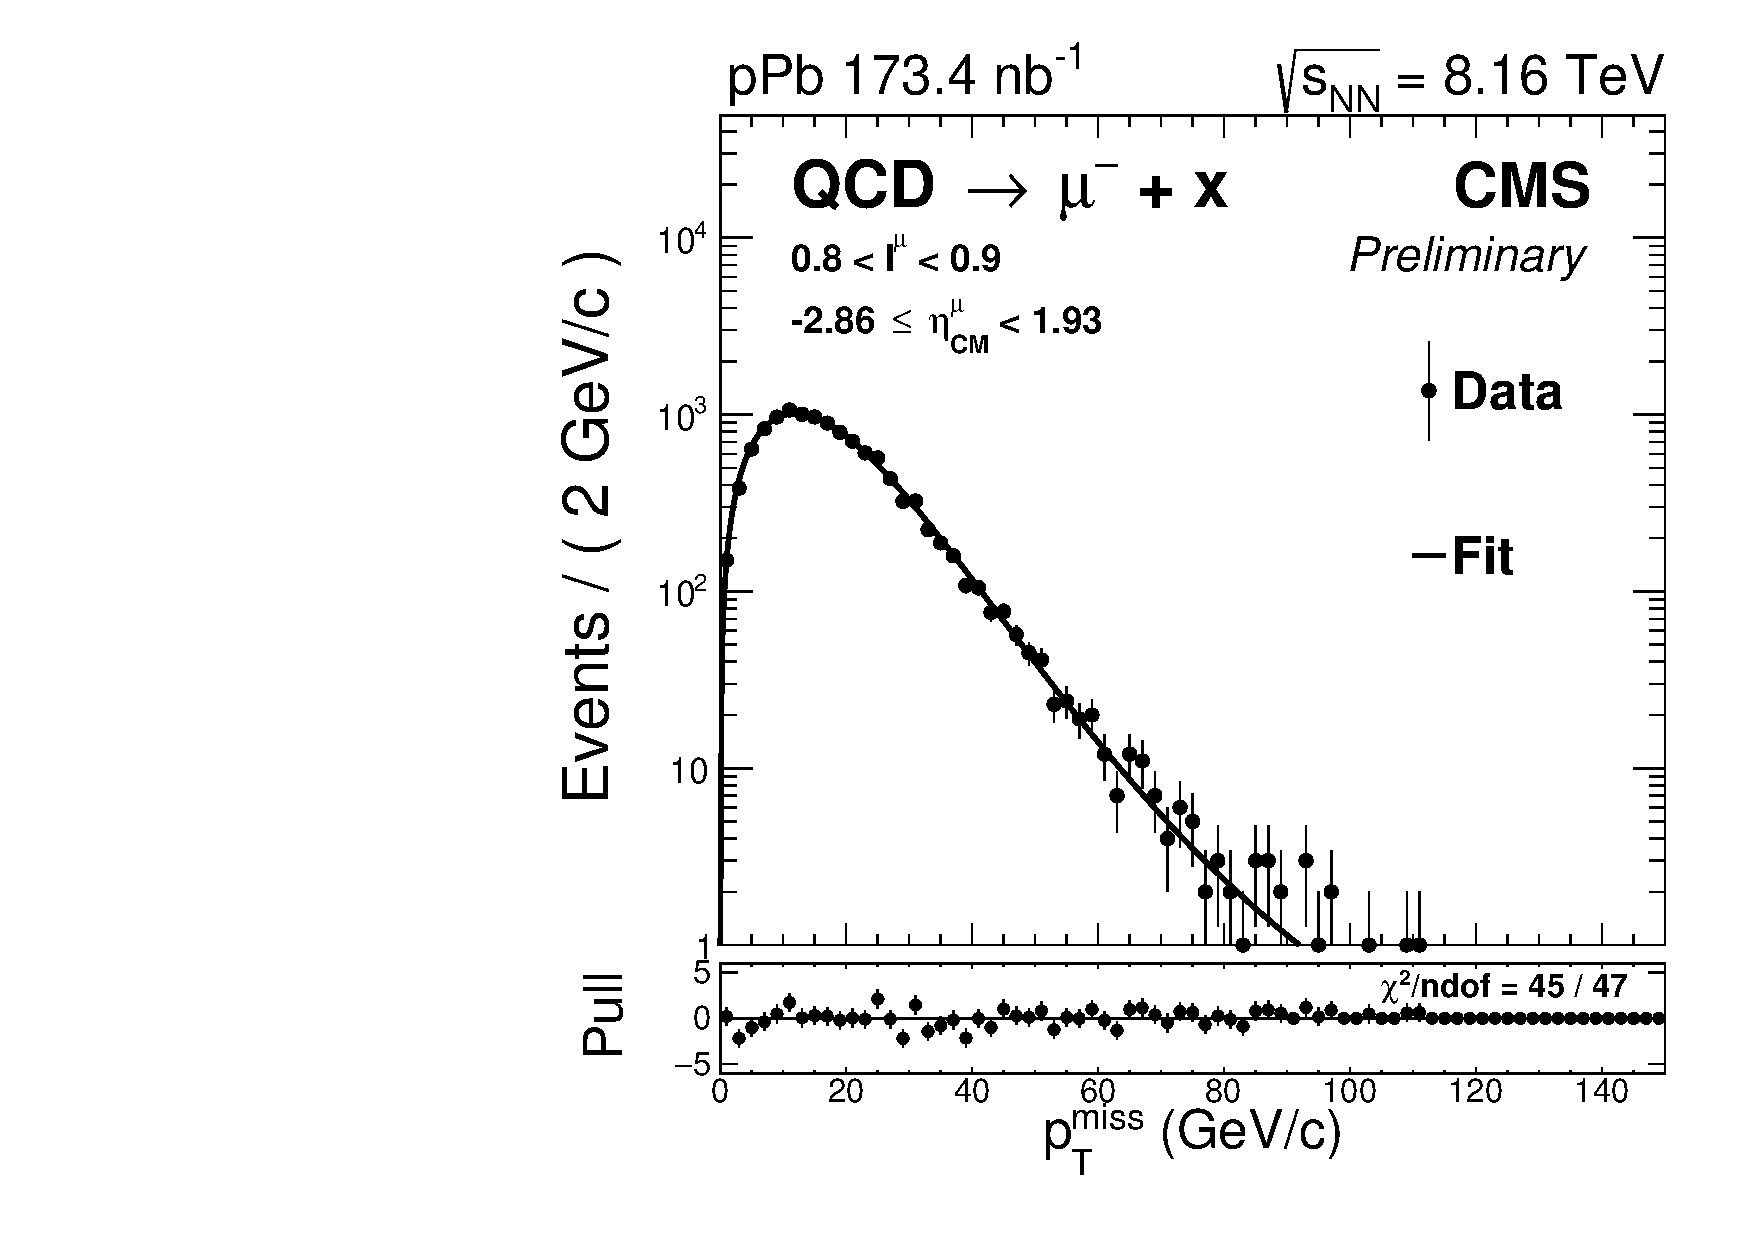
\includegraphics[width=0.45\textwidth]{Figures/WBoson/Analysis/SignalExtraction/QCD_Template/DATA/PLOT_MET_DATA_QCDToMuMi_PA_Model_ModifiedRayleigh_MuEtaCM_-286_193_MuIso_80_90.pdf}\\
  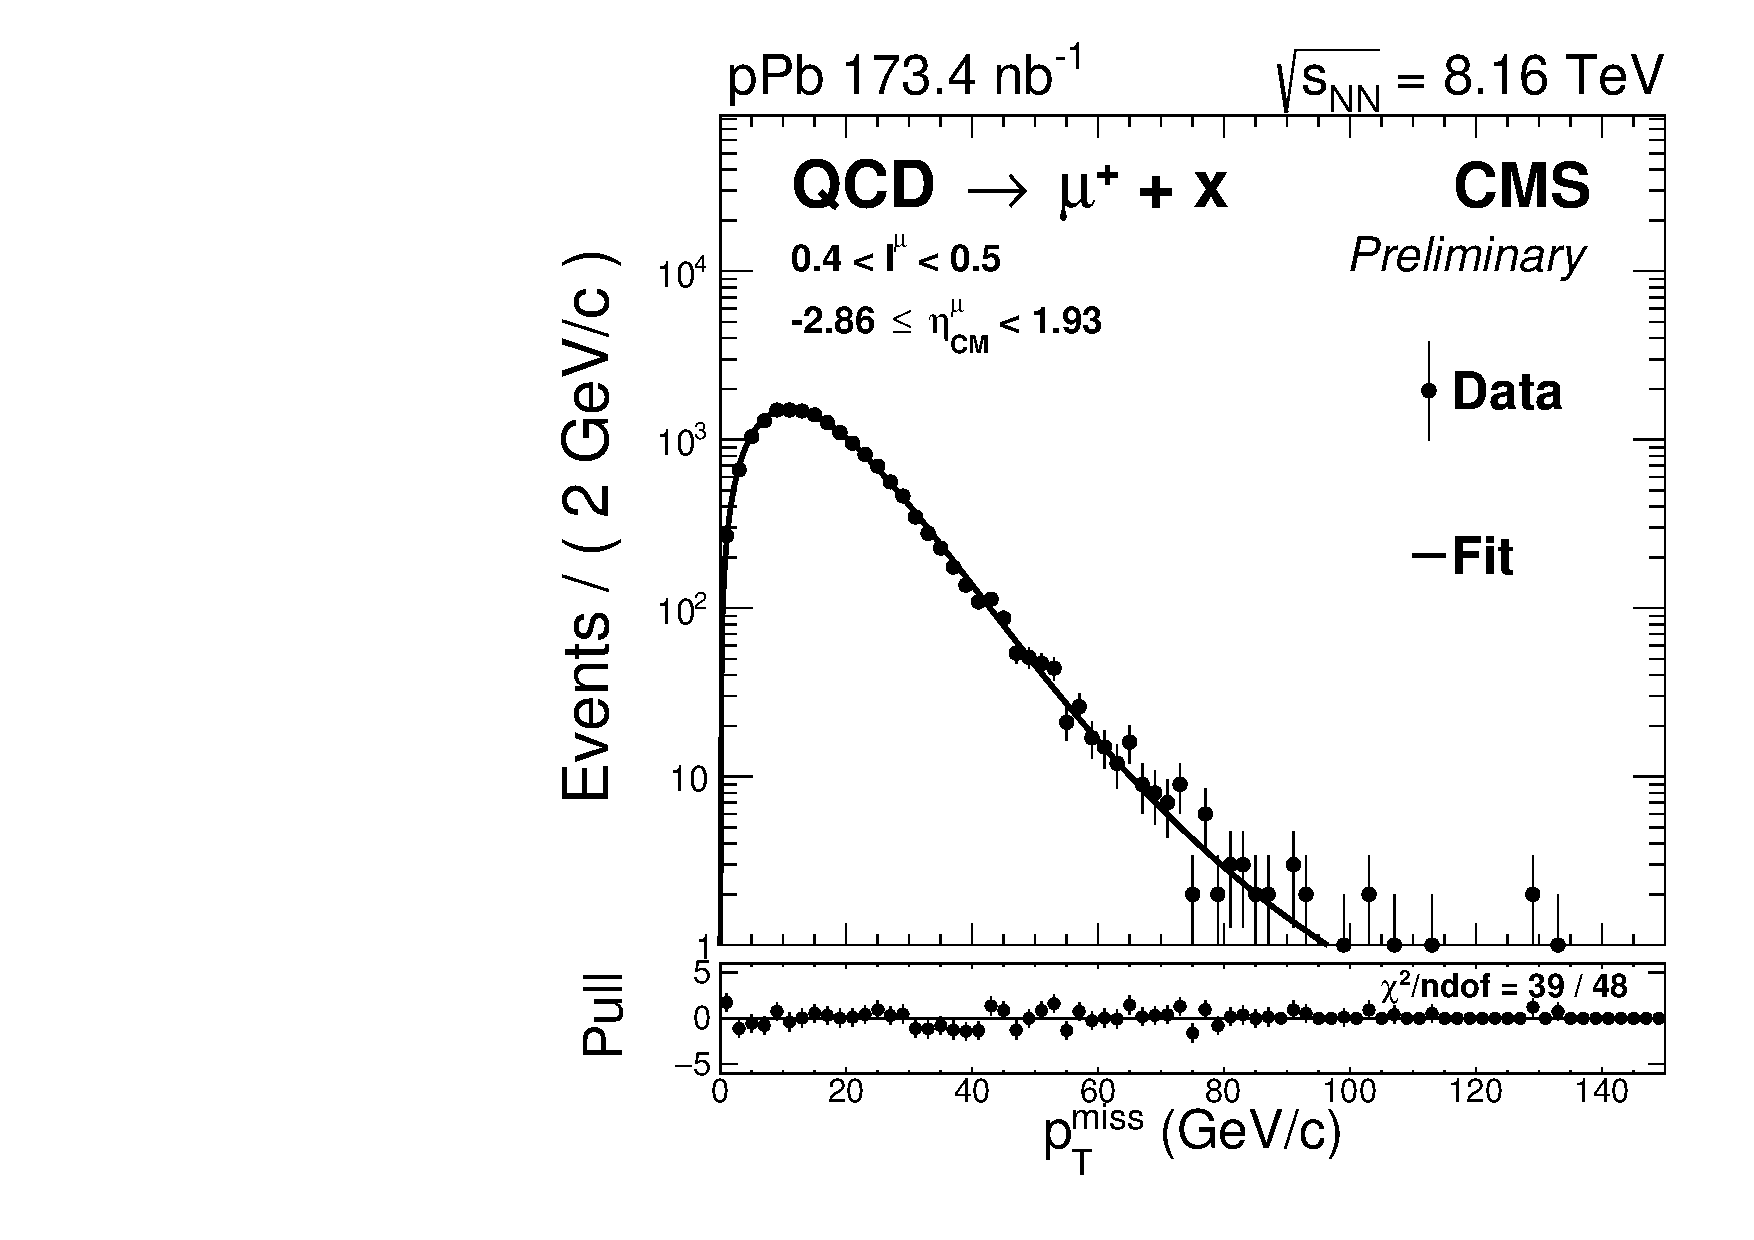
\includegraphics[width=0.45\textwidth]{Figures/WBoson/Analysis/SignalExtraction/QCD_Template/DATA/PLOT_MET_DATA_QCDToMuPl_PA_Model_ModifiedRayleigh_MuEtaCM_-286_193_MuIso_40_50.pdf}
  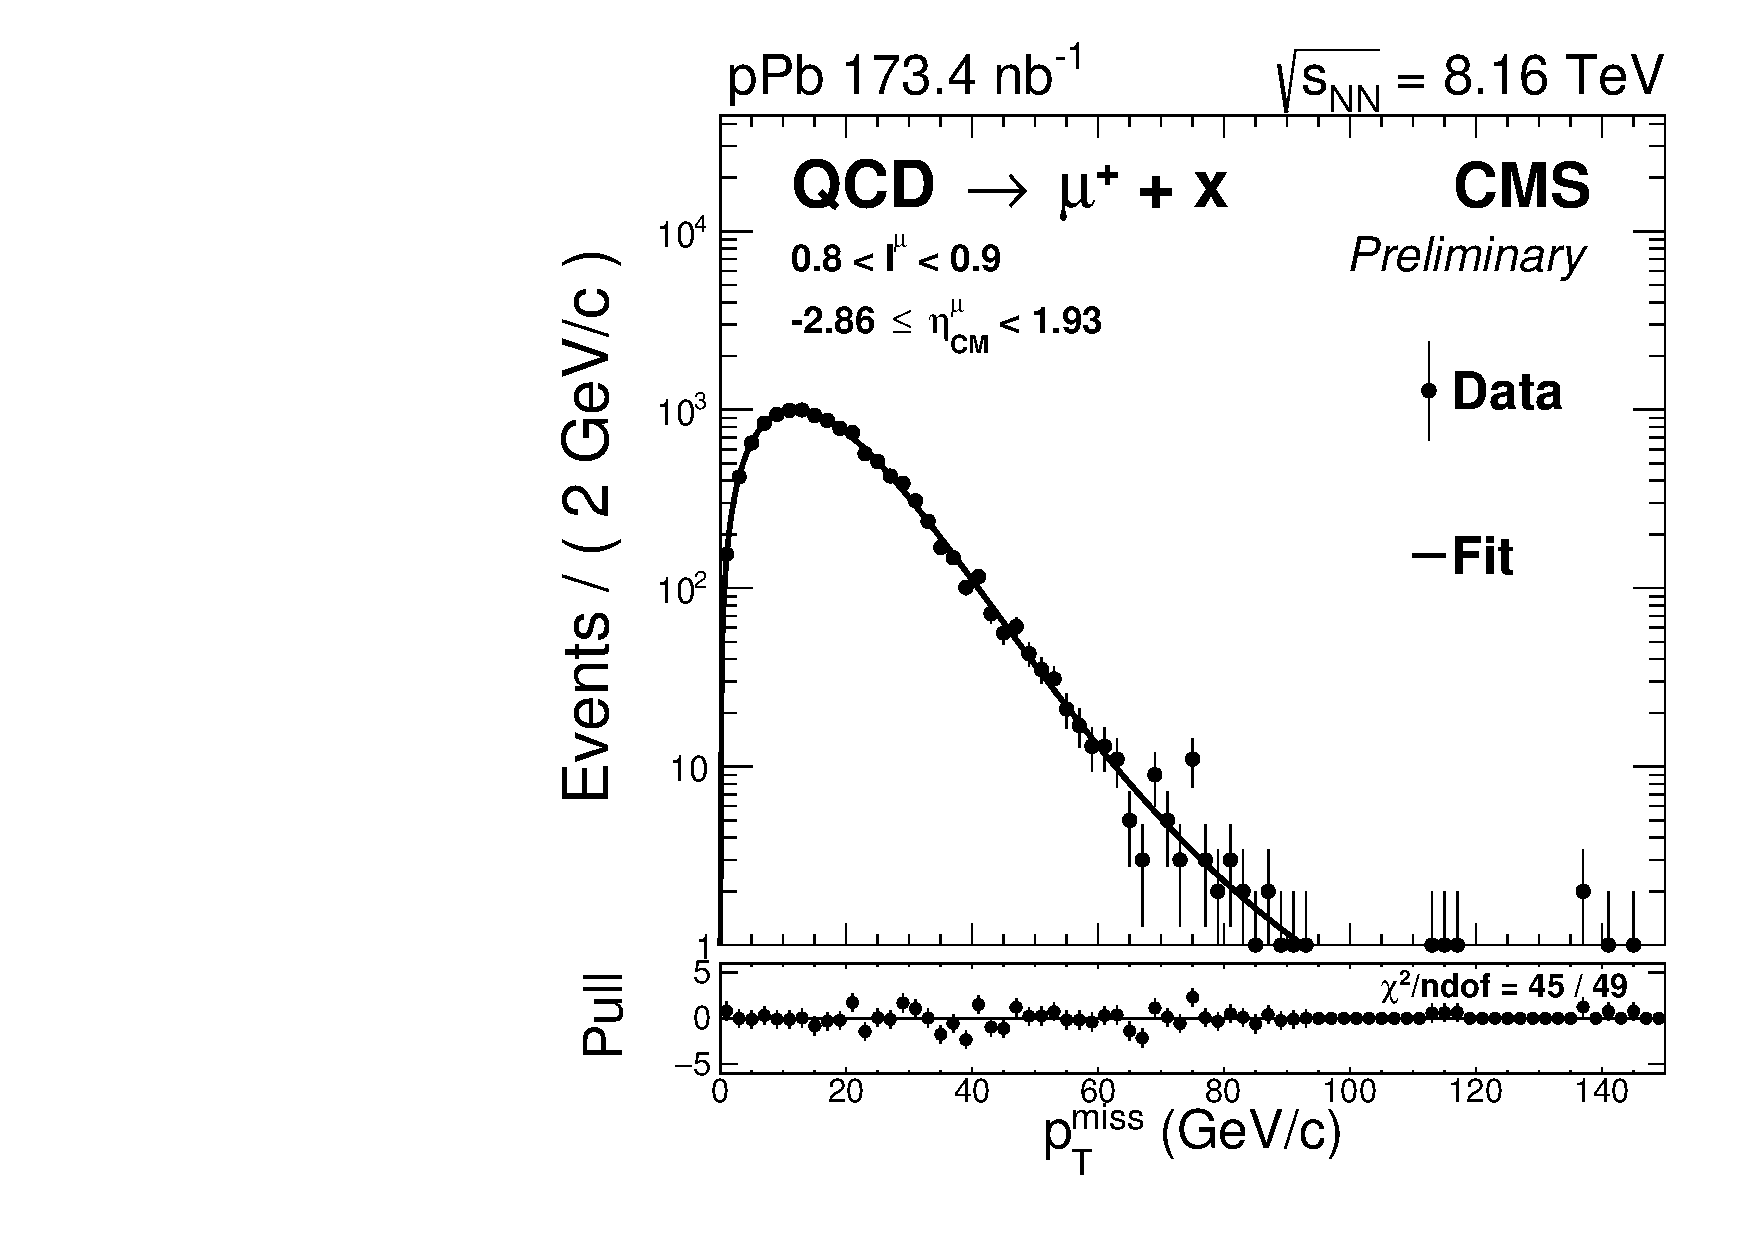
\includegraphics[width=0.45\textwidth]{Figures/WBoson/Analysis/SignalExtraction/QCD_Template/DATA/PLOT_MET_DATA_QCDToMuPl_PA_Model_ModifiedRayleigh_MuEtaCM_-286_193_MuIso_80_90.pdf}
 \caption{QCD jet background fits to the \ptmiss distribution in a control sample of non-isolated muon events  corresponding to the muon isolation bins: $0.4 < \iso < 0.5$ (left) and $0.8 < \iso < 0.9$ (right). The results are shown for positive (top) and negative (bottom) charged muons separately.}
 \label{fig:QCD_Fits}
\end{figure}

The QCD background parameters $\sigma_{0}$, $\sigma_{1}$, and $\sigma_{2}$, are extracted from the fits to the \ptmiss spectrum in each muon isolation bin, and their profile as a function of \iso is observed to be well described by a linear function, given by:

\begin{equation}
 \sigma_{i}\left(\iso\right) = \hat{\sigma}_{i} + s_{i}{\cdot}\iso
\end{equation}

where $\hat{\sigma}_{i}$ and $s_{i}$ are free parameters extracted separately for each QCD background parameter. The outcome of the linear fits is shown in \fig{fig:QCD_Extrapolation}.

\begin{figure}[htb!]
 \centering
 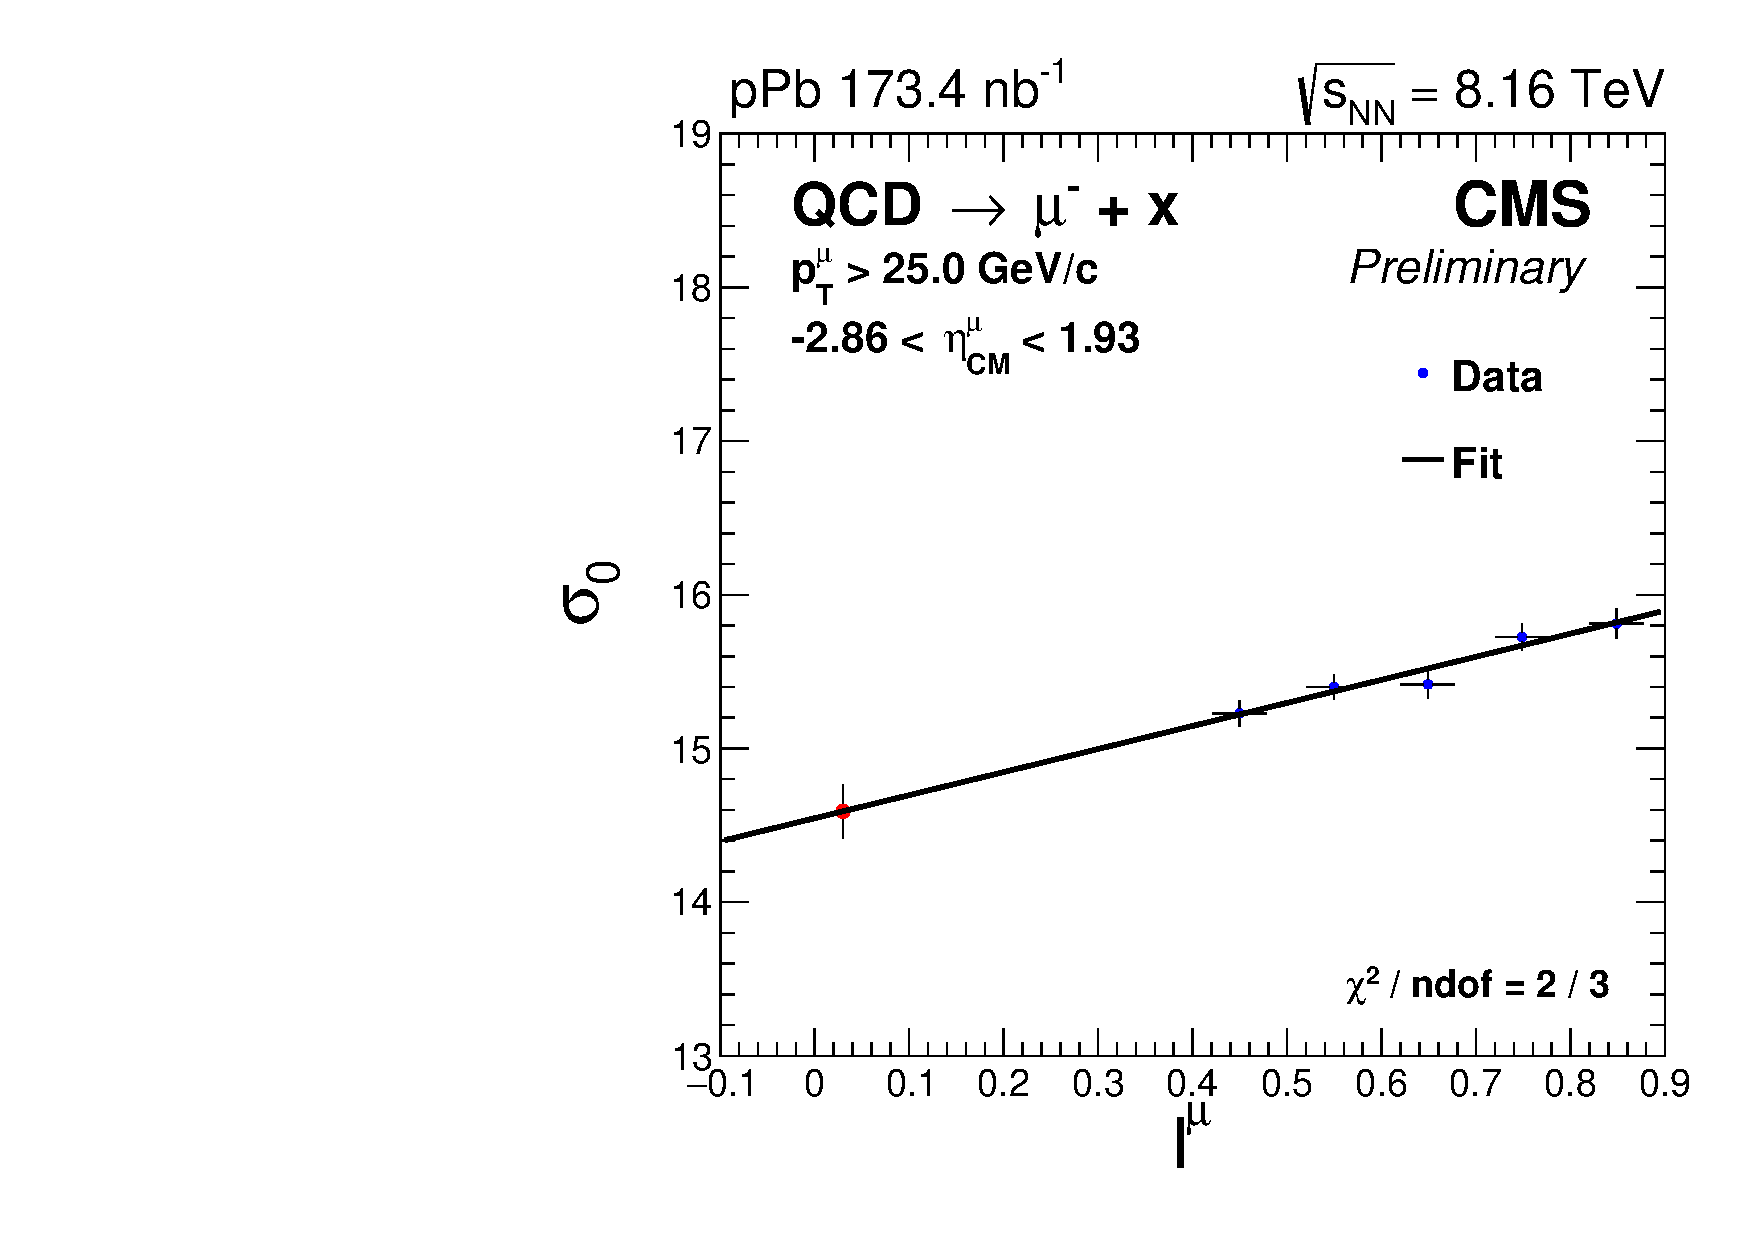
\includegraphics[width=0.32\textwidth]{Figures/WBoson/Analysis/SignalExtraction/QCD_Template/EXTRAPOLATION/graph_Sigma0_QCDToMuMi_PA_-29_eta_19_250_pt_1000000.pdf}
 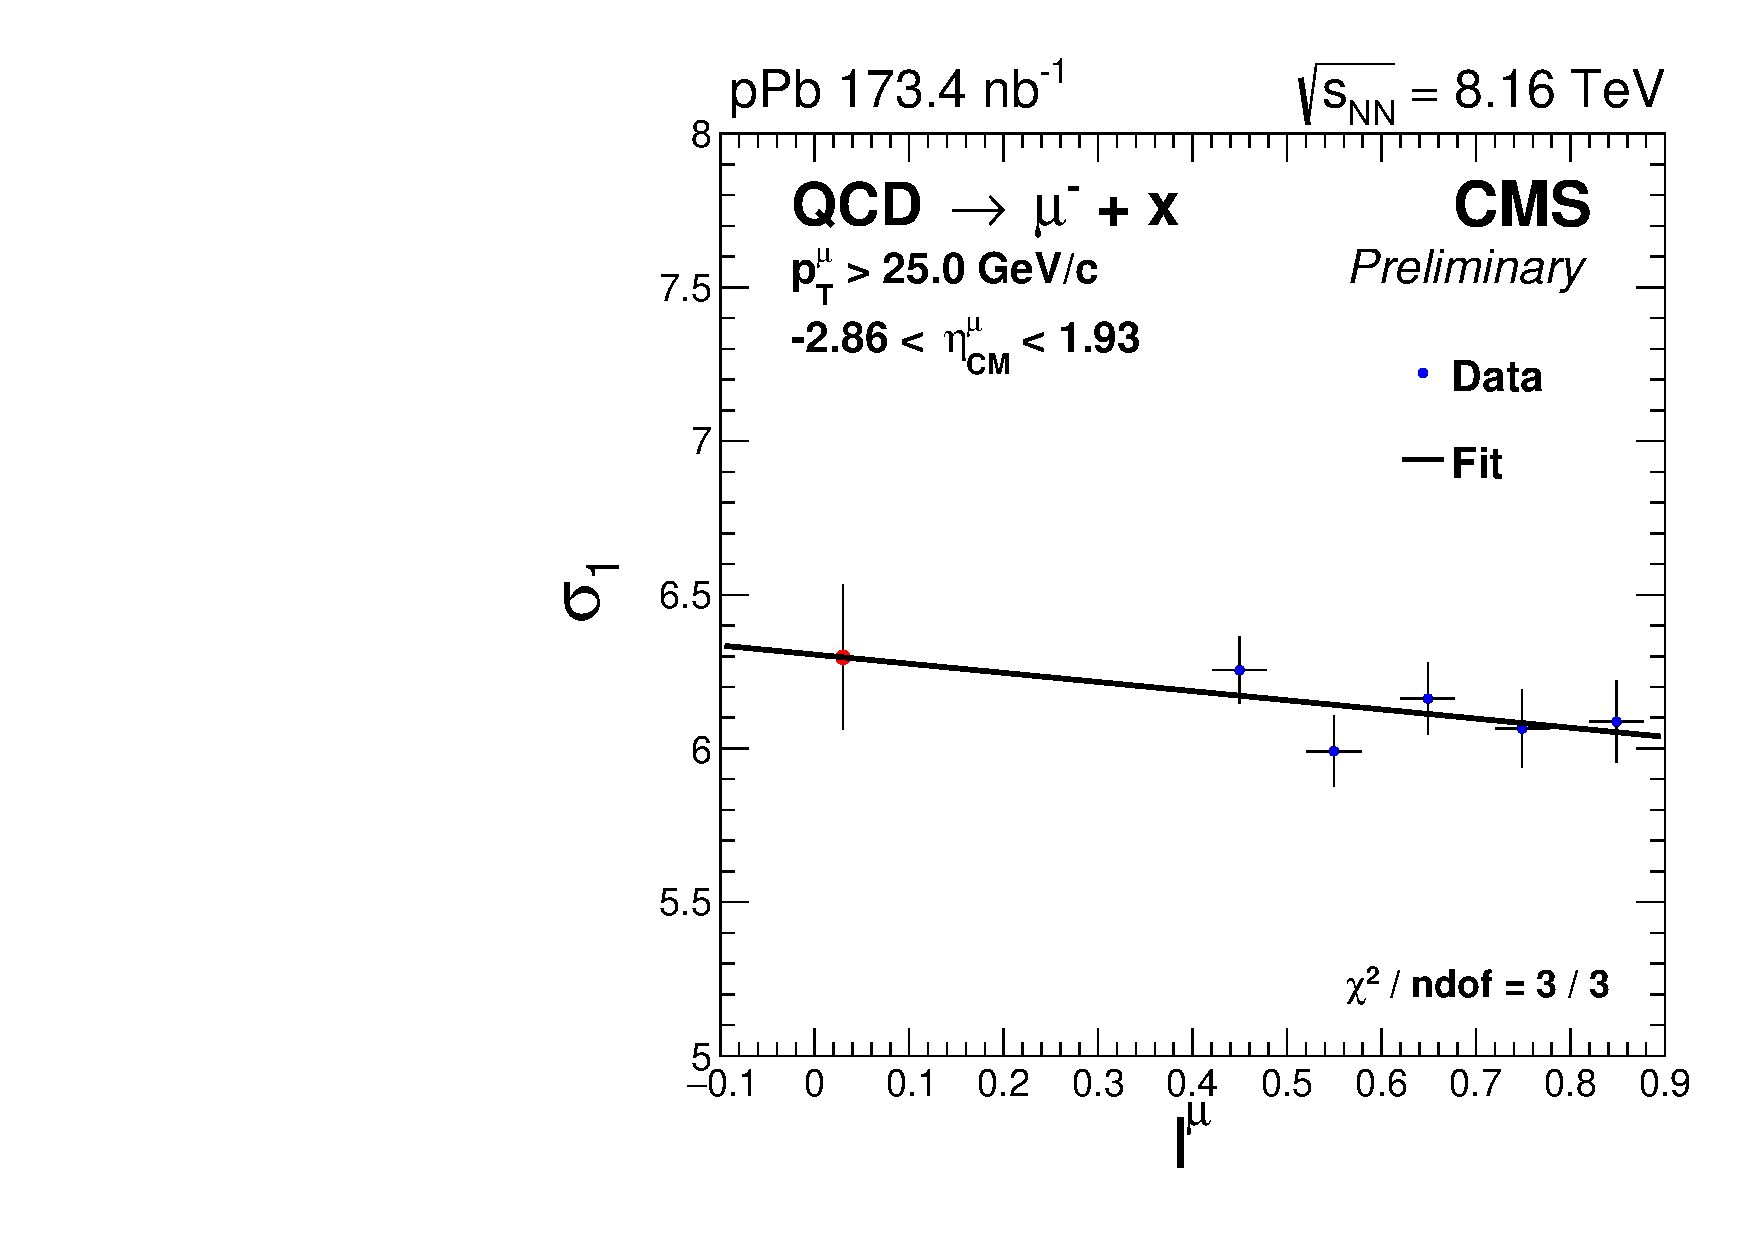
\includegraphics[width=0.32\textwidth]{Figures/WBoson/Analysis/SignalExtraction/QCD_Template/EXTRAPOLATION/graph_Sigma1_QCDToMuMi_PA_-29_eta_19_250_pt_1000000.pdf}
 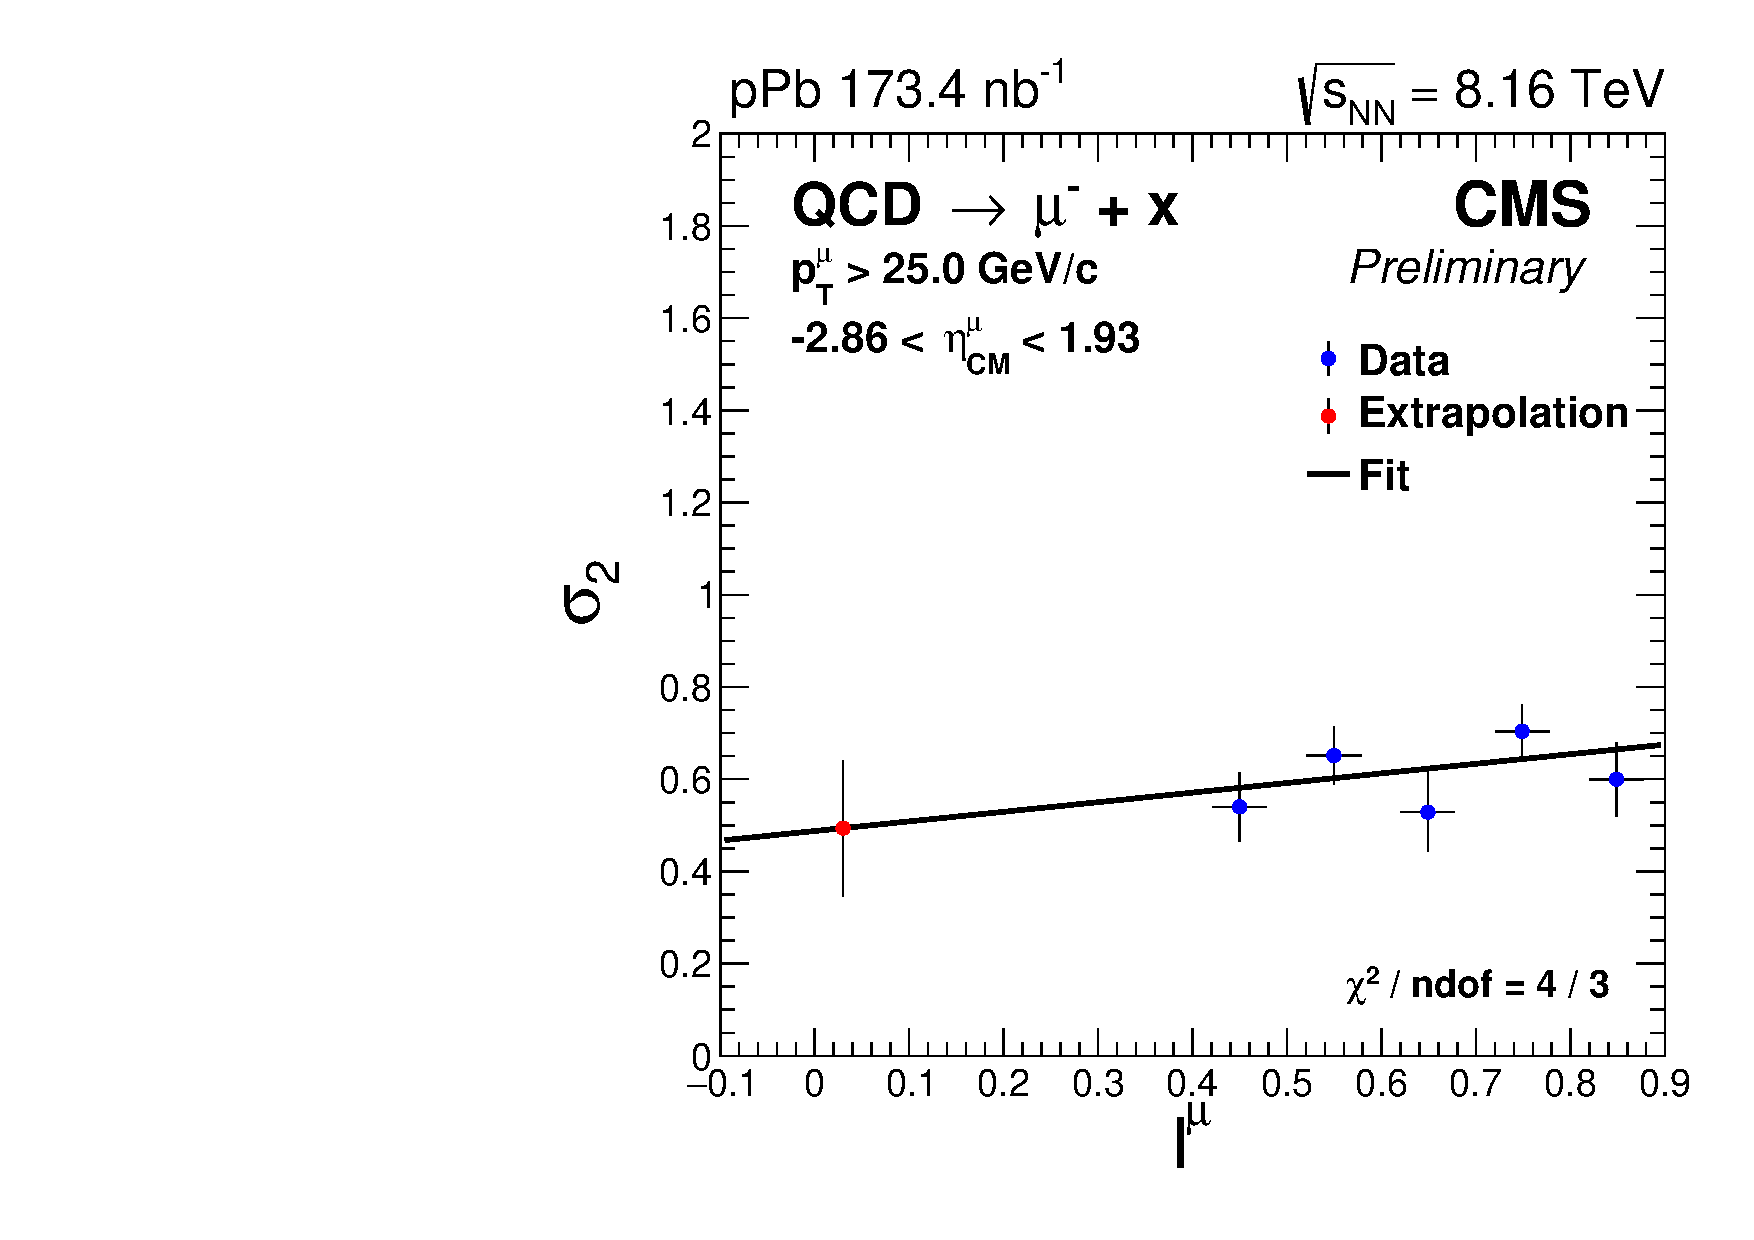
\includegraphics[width=0.32\textwidth]{Figures/WBoson/Analysis/SignalExtraction/QCD_Template/EXTRAPOLATION/graph_Sigma2_QCDToMuMi_PA_-29_eta_19_250_pt_1000000.pdf}
%%
 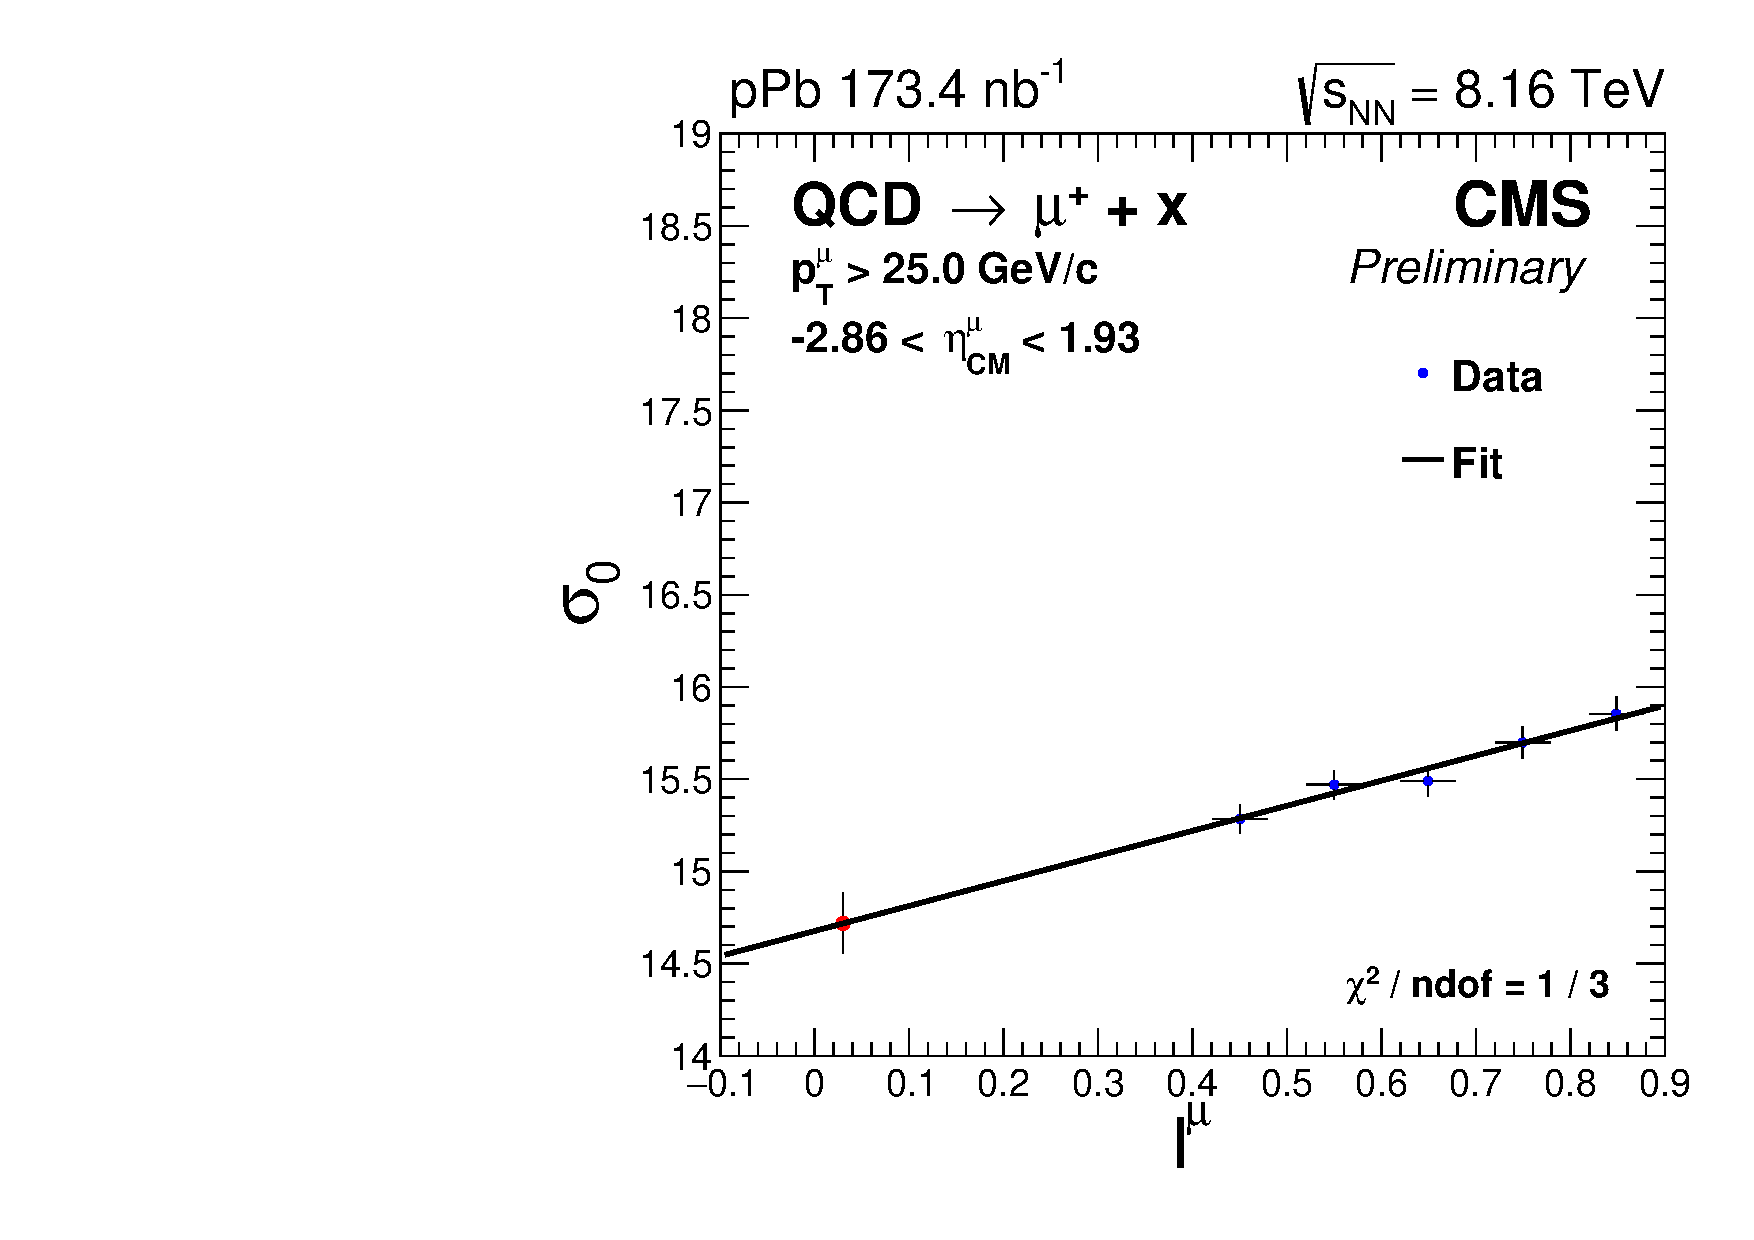
\includegraphics[width=0.32\textwidth]{Figures/WBoson/Analysis/SignalExtraction/QCD_Template/EXTRAPOLATION/graph_Sigma0_QCDToMuPl_PA_-29_eta_19_250_pt_1000000.pdf}
 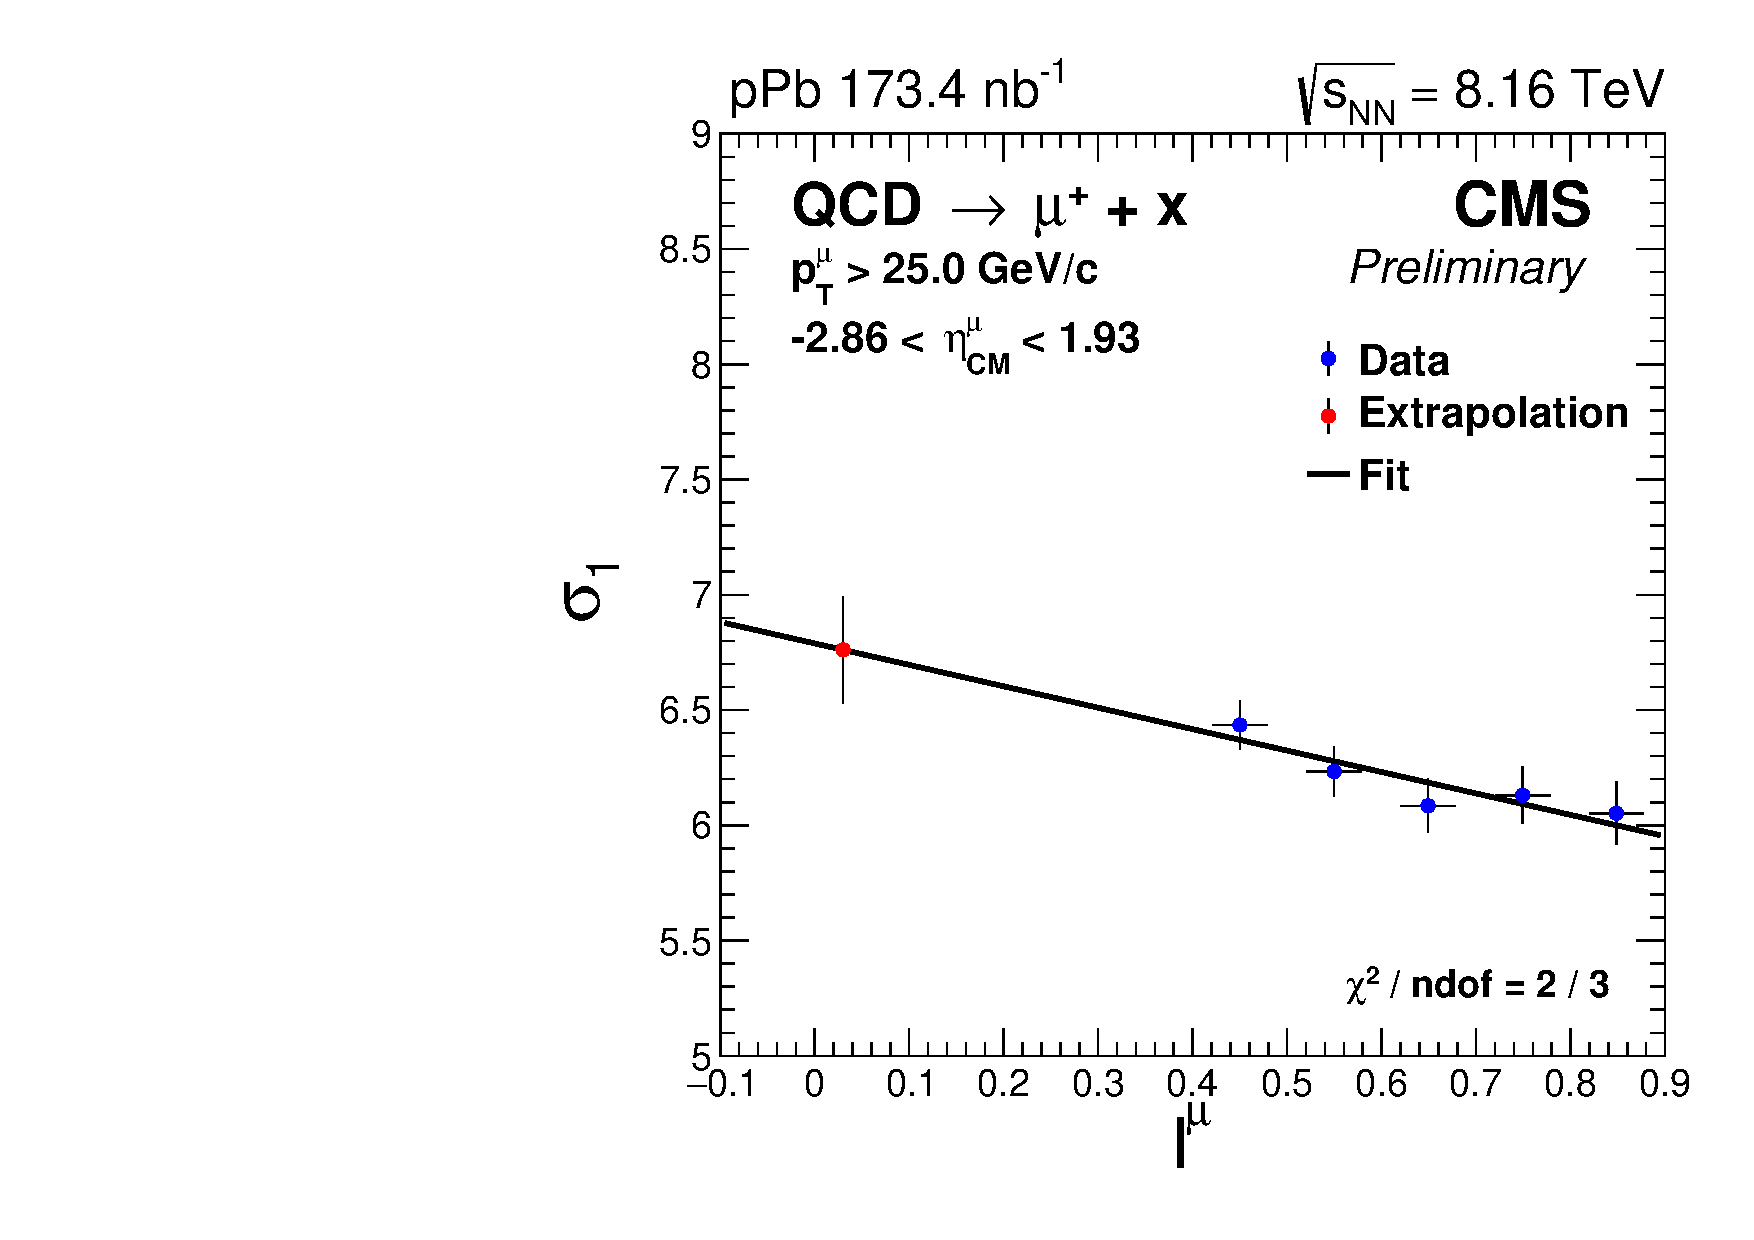
\includegraphics[width=0.32\textwidth]{Figures/WBoson/Analysis/SignalExtraction/QCD_Template/EXTRAPOLATION/graph_Sigma1_QCDToMuPl_PA_-29_eta_19_250_pt_1000000.pdf}
 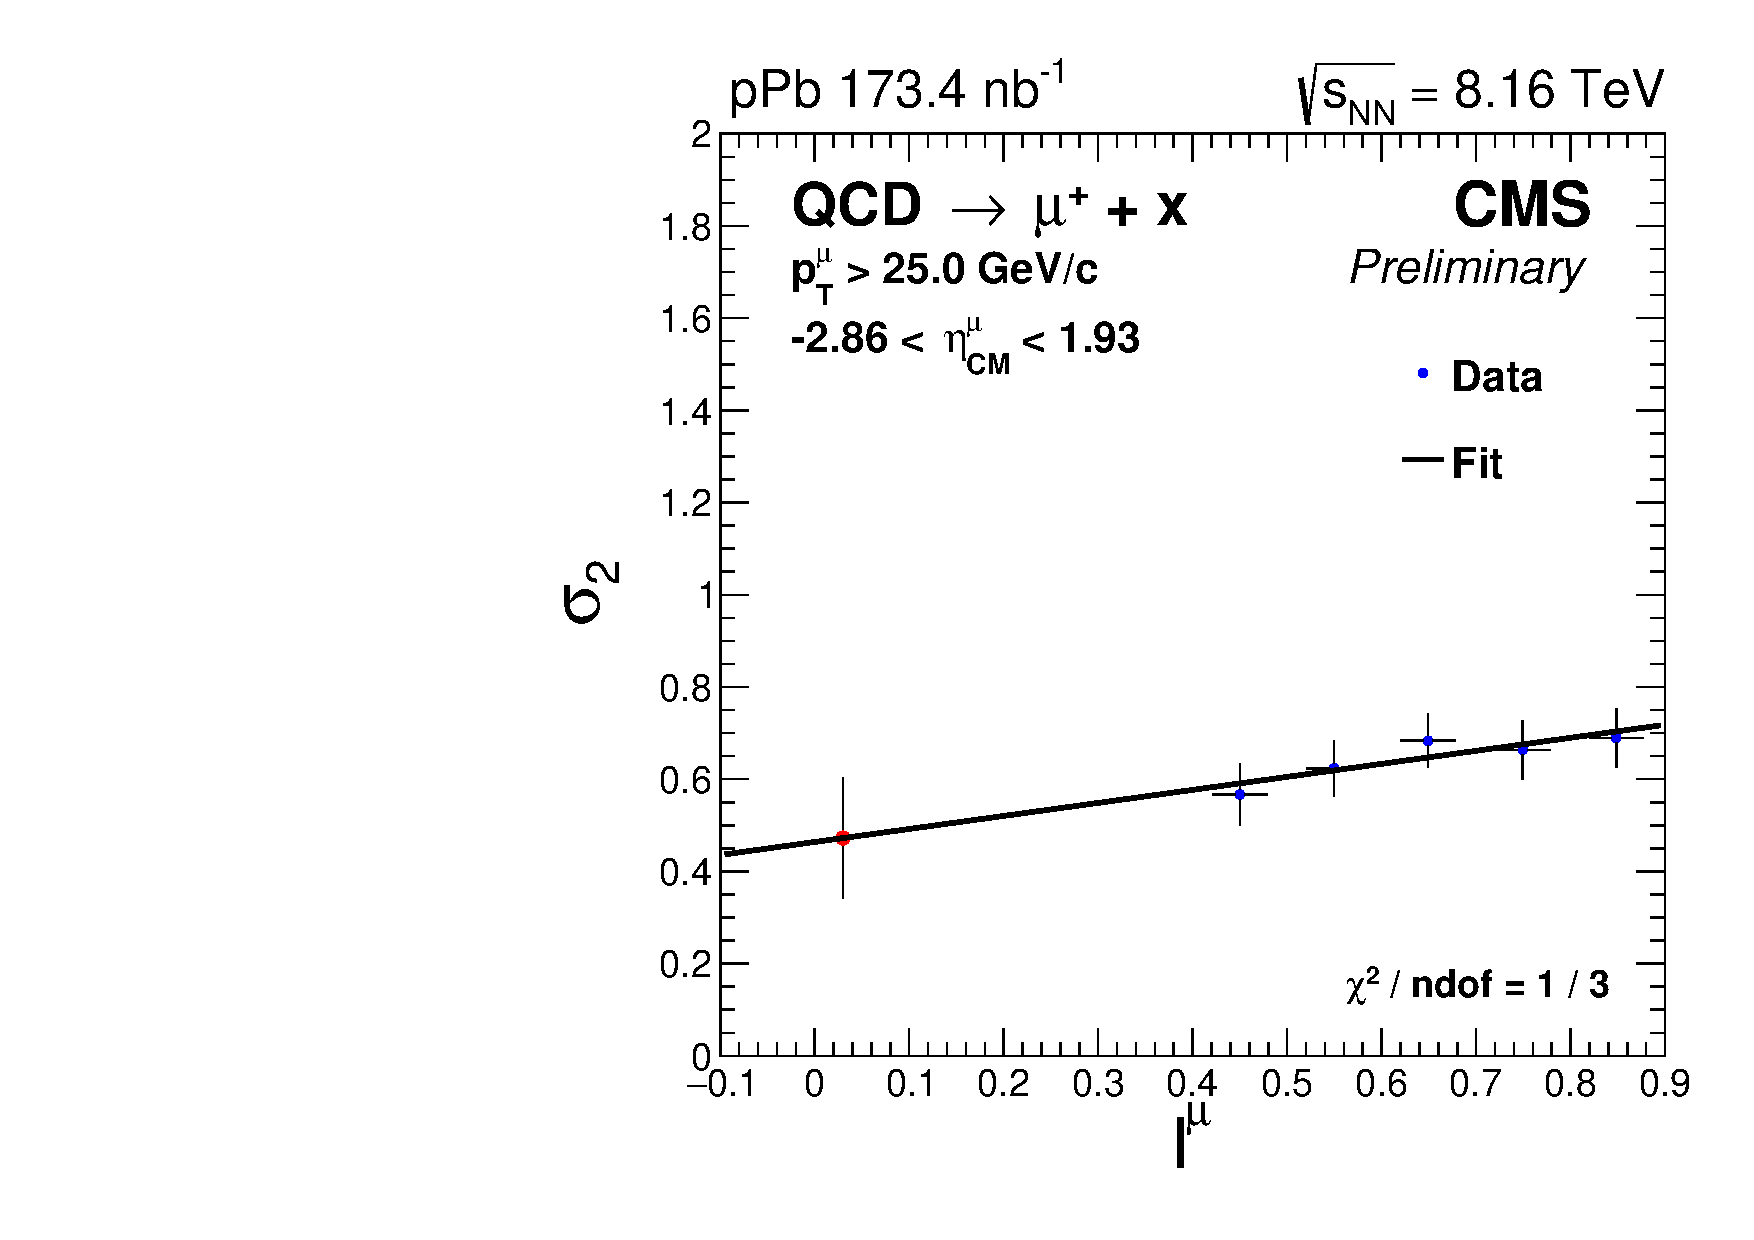
\includegraphics[width=0.32\textwidth]{Figures/WBoson/Analysis/SignalExtraction/QCD_Template/EXTRAPOLATION/graph_Sigma2_QCDToMuPl_PA_-29_eta_19_250_pt_1000000.pdf}
 \caption{Linear fits to the profile of the QCD background parameters: $\sigma_{0}$ (left), $\sigma_{1}$ (middle) and $\sigma_{2}$ (right), with respect to the muon isolation variable \iso. The results are shown for negative (top) and positive (bottom) charged muons in the \etaMuCM-inclusive range. The red points represents the value obtained by linearly extrapolating to $\iso = 0.03$.}
 \label{fig:QCD_Extrapolation}
\end{figure}

The $\sigma_{0}$, $\sigma_{1}$, and $\sigma_{2}$ parameters are extrapolated to the signal region (average muon isolation of 0.03) using the parametrisation as a function of \iso extracted from the linear fits. The values of the QCD background parameters derived from the extrapolation are presented in \tab{tab:QCD_Extrapolation}.

\begin{table}[htb!]
 \centering
 \begin{tabular}{|c|c|c|}\hline
   Parameter & $\text{QCD jet} \to \mu^{-}$ & $\text{QCD jet} \to \mu^{+}$ \\\hline
   $\sigma_{0}$ & 14.6$\pm$0.2 & 14.7$\pm$0.2 \\\hline
   $\sigma_{1}$ & 6.3$\pm$0.2 & 6.8$\pm$0.2 \\\hline
   $\sigma_{2}$ & 0.5$\pm$0.2 & 0.5$\pm$0.1 \\\hline
 \end{tabular}
 \caption{QCD background parameters extrapolated to $\iso = 0.03$. The results are presented for positive and negative charged muons in the \etaMuCM-inclusive range.}
 \label{tab:QCD_Extrapolation}
\end{table}

The QCD jet \ptmiss distribution is estimated separately for positive and negative charged muon events to account for possible differences between the $\mu^{+}$ and $\mu^{-}$ yields arising from the detector response, acceptance and/or muon production from hadron decays. Although the differences are expected to be small, they are still computed separately to be conservative.

The dependence of the extrapolated \ptmiss functional form of the QCD jet background on the muon \etaMuCM is checked by splitting the control sample in different \etaMuCM bins, and then repeating the QCD jet shape extraction procedure for each \etaMuCM bin. The results of the extrapolated values of $\sigma_{0}$, $\sigma_{1}$, and $\sigma_{2}$, determined for each \etaMuCM bin, are compared in \fig{fig:QCD_Extrapolation_Eta} to the results obtained in the \etaMuCM-inclusive range.

\begin{figure}[htb!]
 \centering
  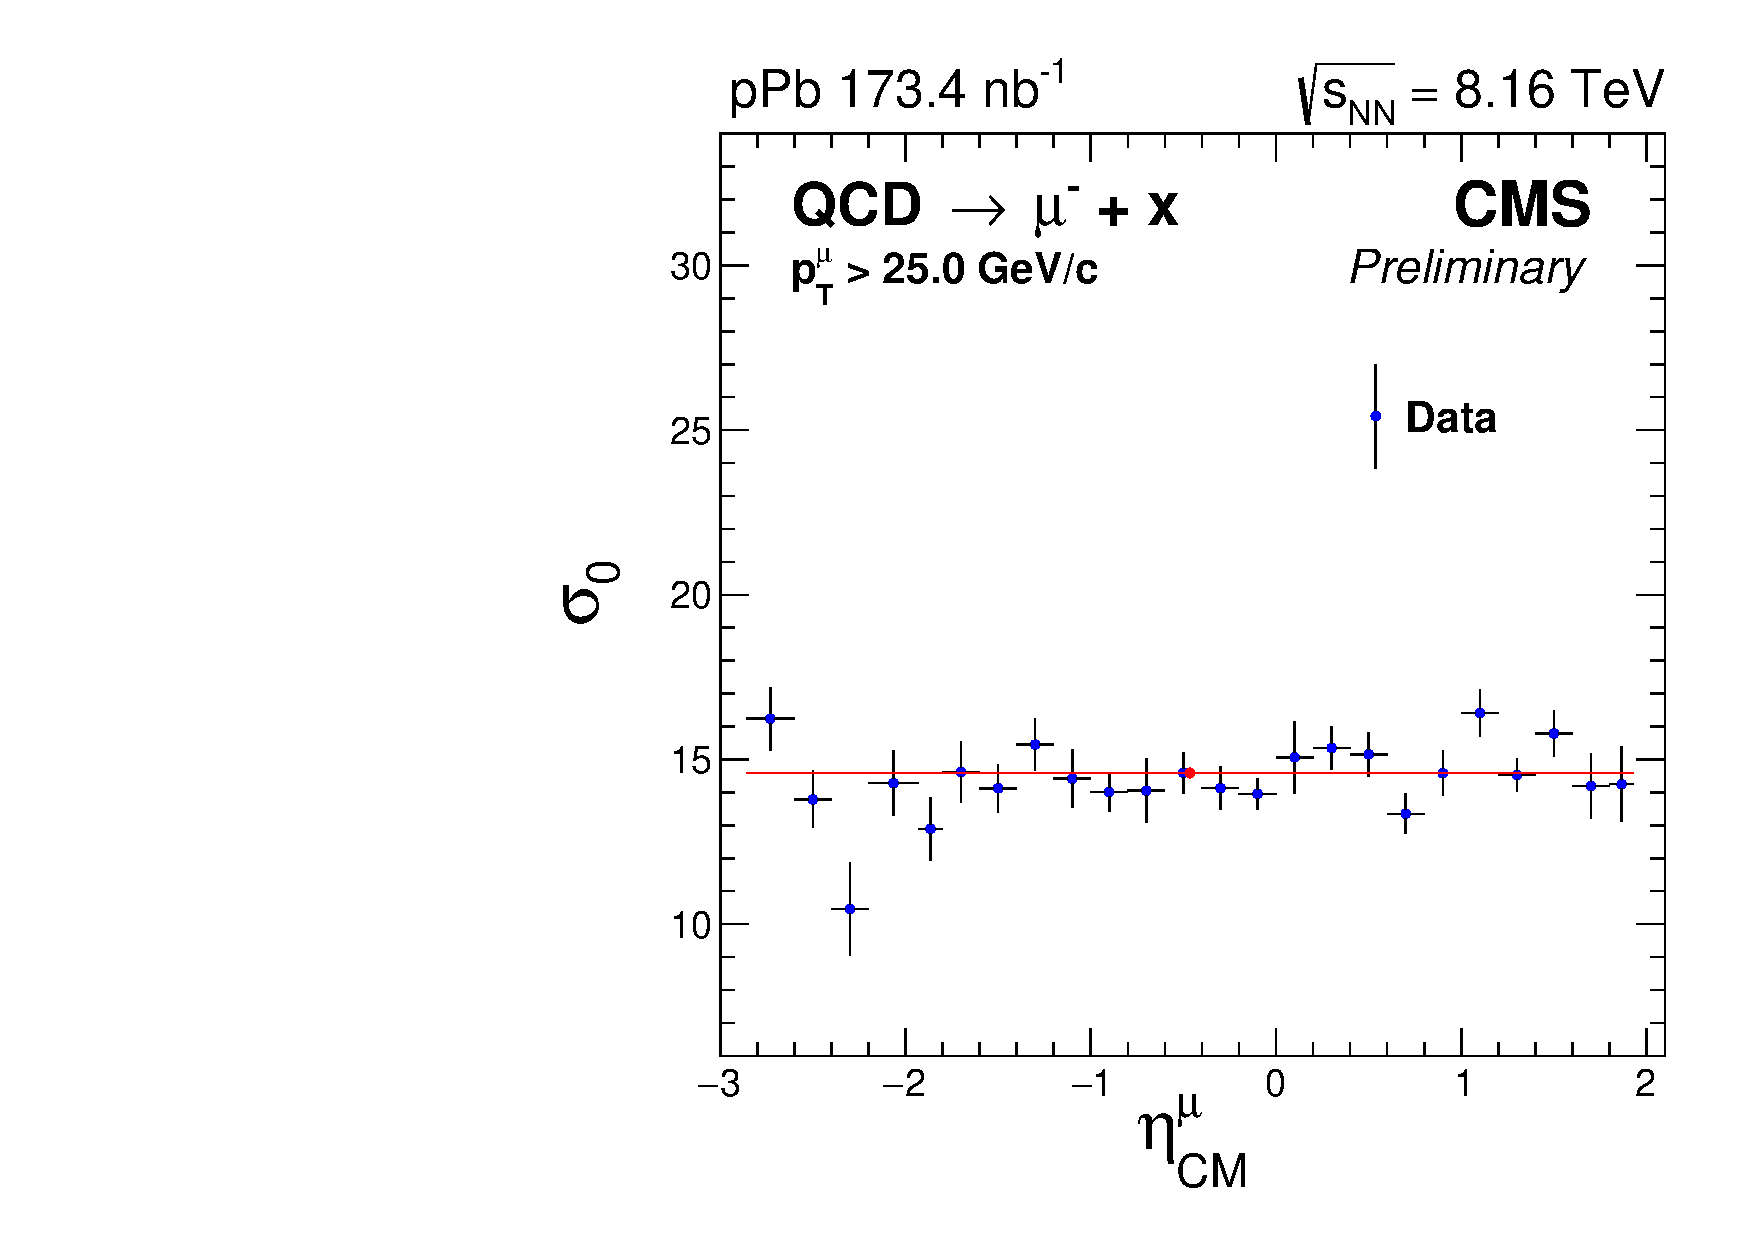
\includegraphics[width=0.32\textwidth]{Figures/WBoson/Analysis/SignalExtraction/QCD_Template/EXTRAPOLATION_ETA/exGraph_ETA_Sigma0_QCDToMuMi_PA.pdf}
  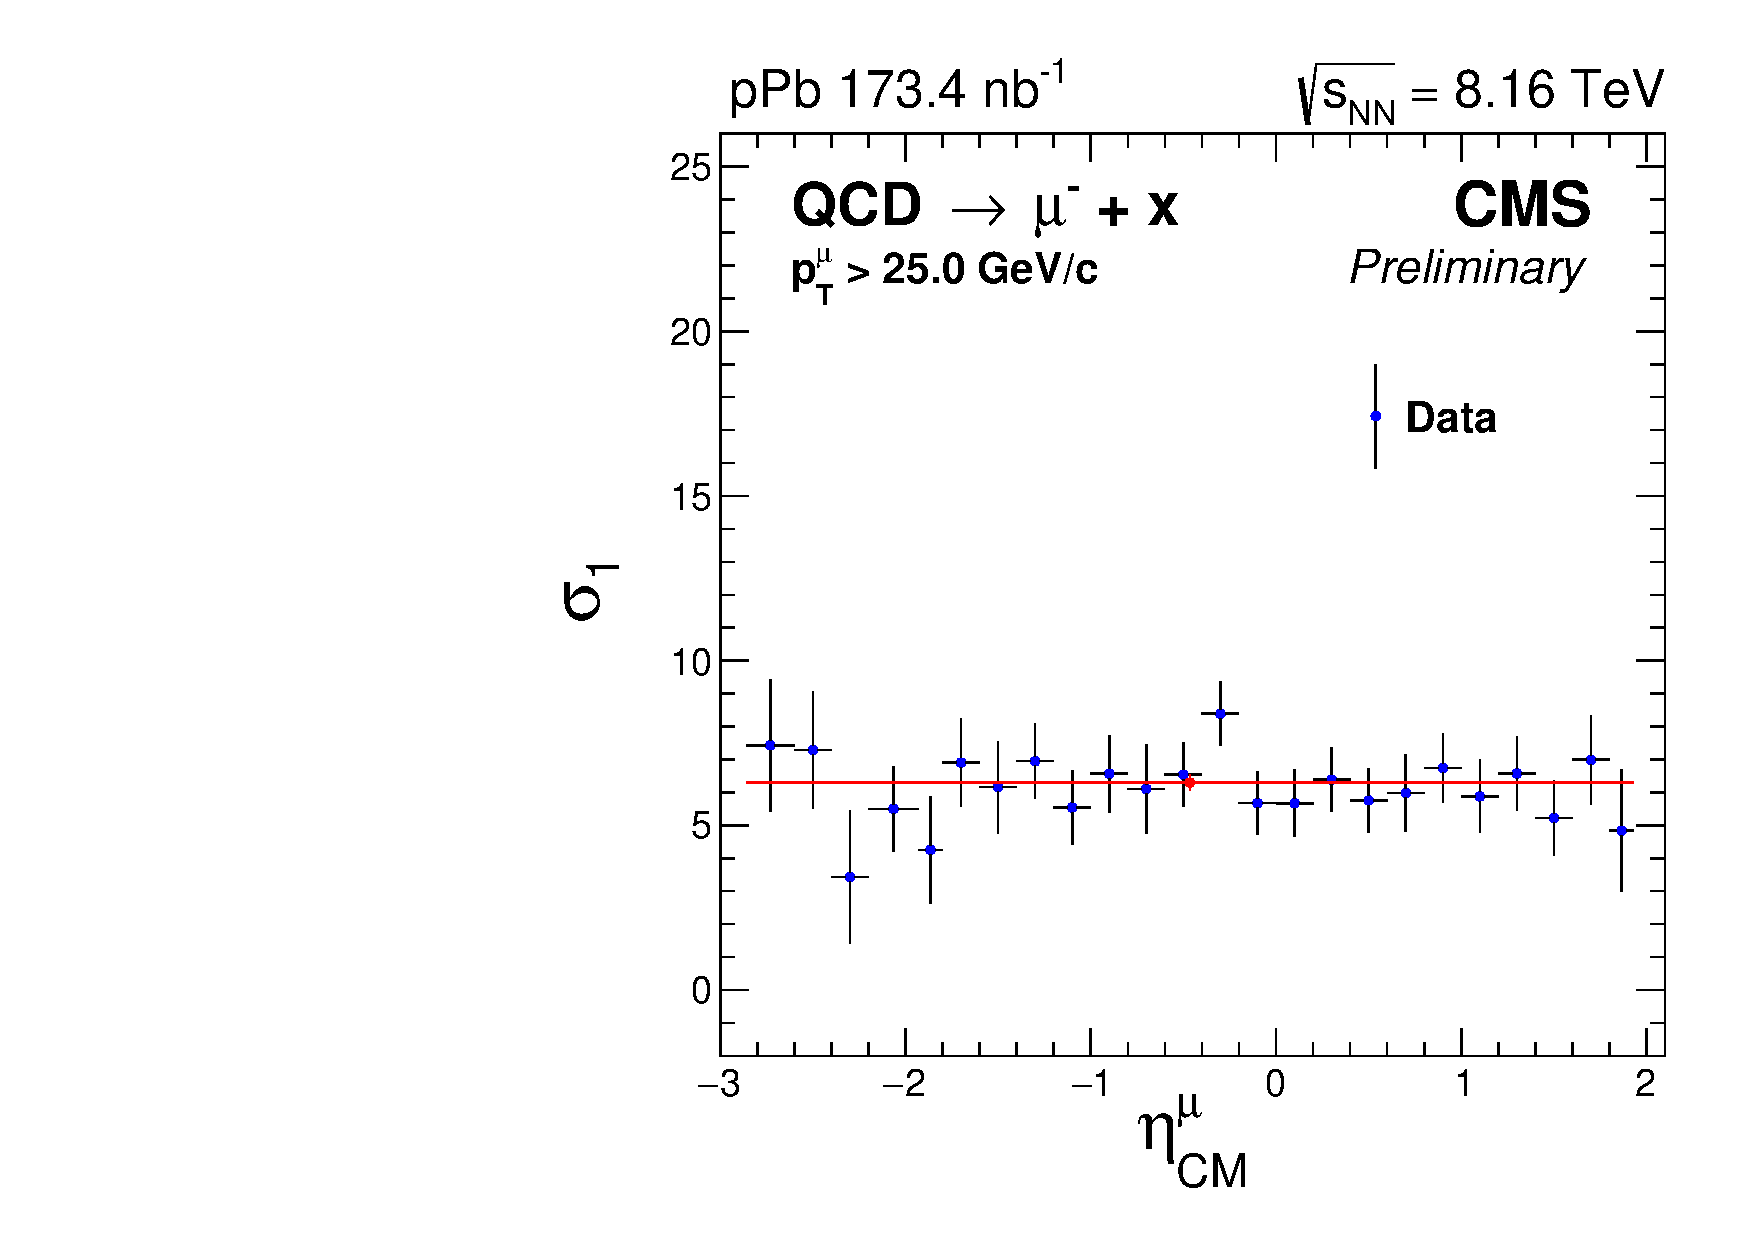
\includegraphics[width=0.32\textwidth]{Figures/WBoson/Analysis/SignalExtraction/QCD_Template/EXTRAPOLATION_ETA/exGraph_ETA_Sigma1_QCDToMuMi_PA.pdf}
  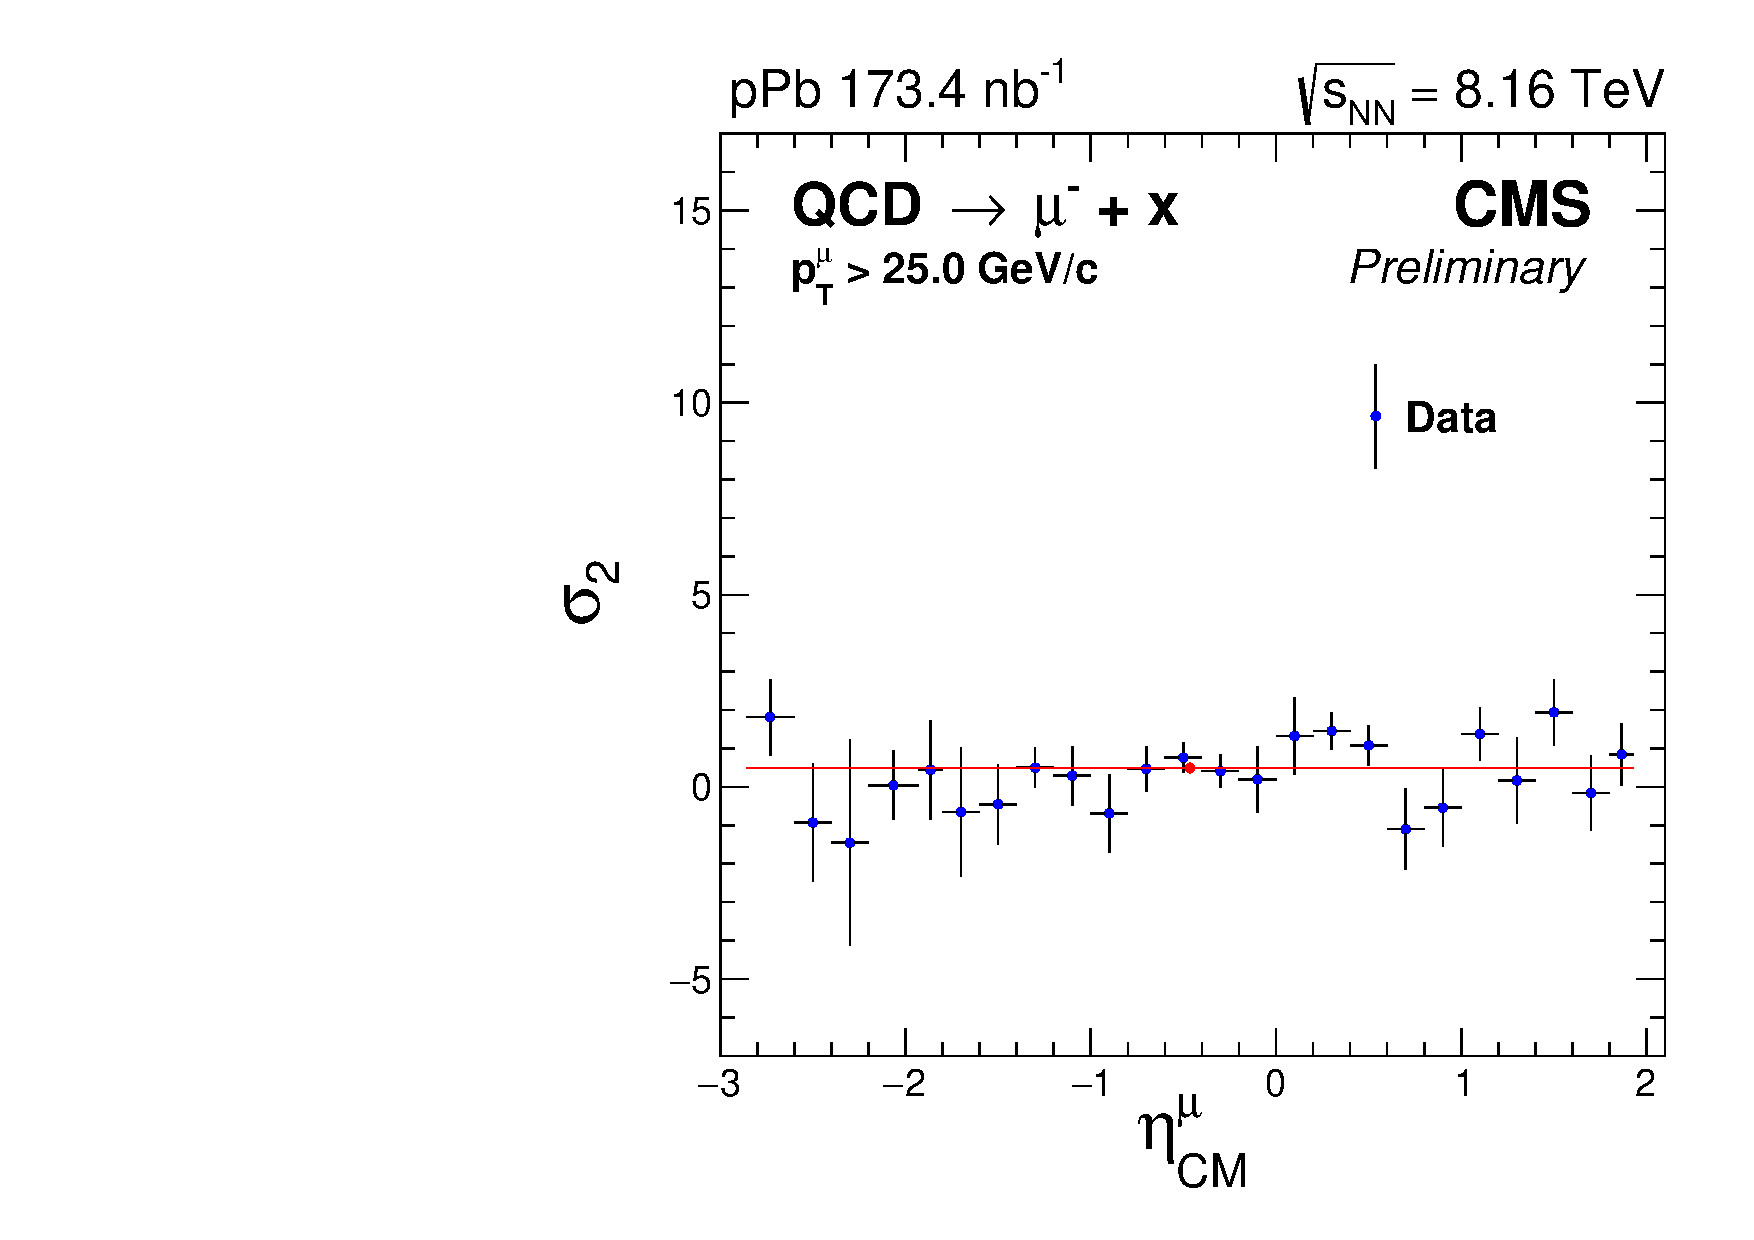
\includegraphics[width=0.32\textwidth]{Figures/WBoson/Analysis/SignalExtraction/QCD_Template/EXTRAPOLATION_ETA/exGraph_ETA_Sigma2_QCDToMuMi_PA.pdf}
%%
  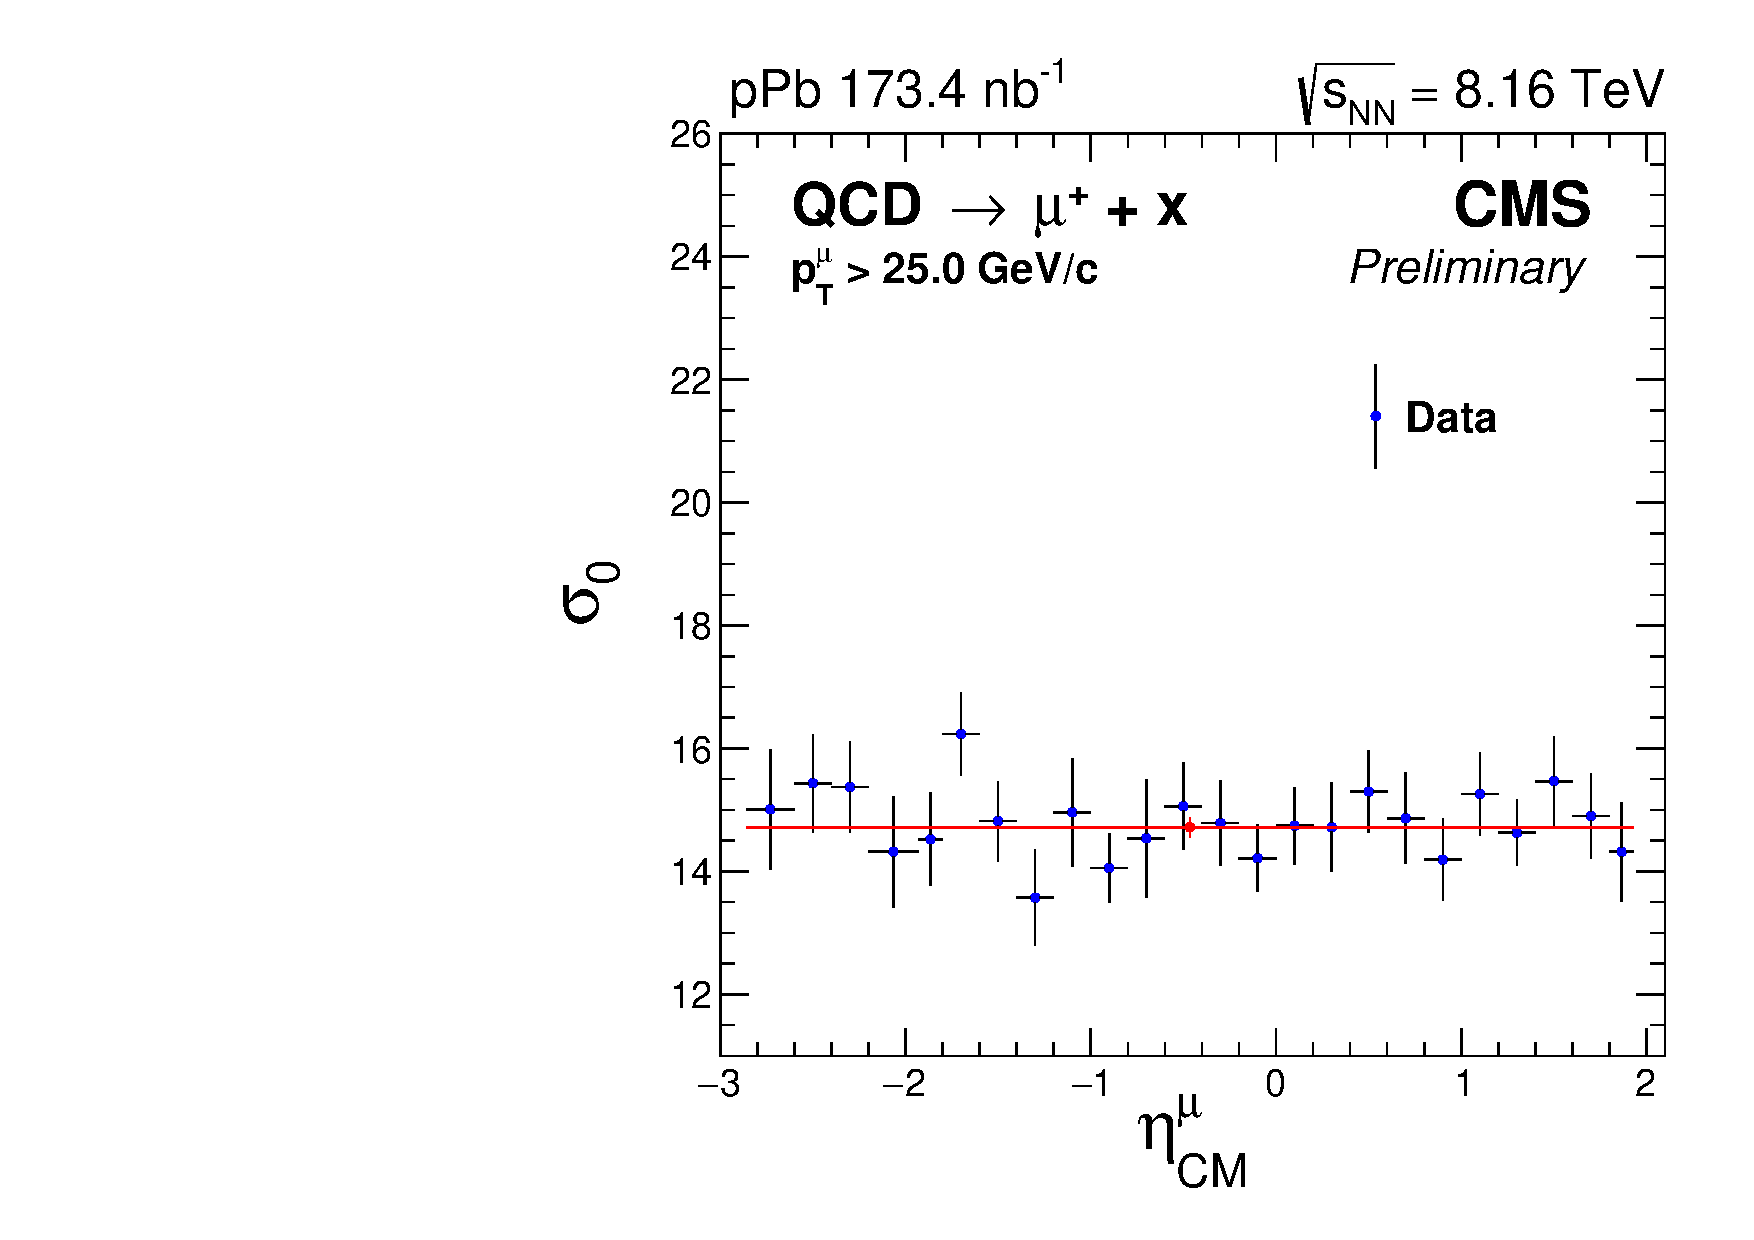
\includegraphics[width=0.32\textwidth]{Figures/WBoson/Analysis/SignalExtraction/QCD_Template/EXTRAPOLATION_ETA/exGraph_ETA_Sigma0_QCDToMuPl_PA.pdf}
  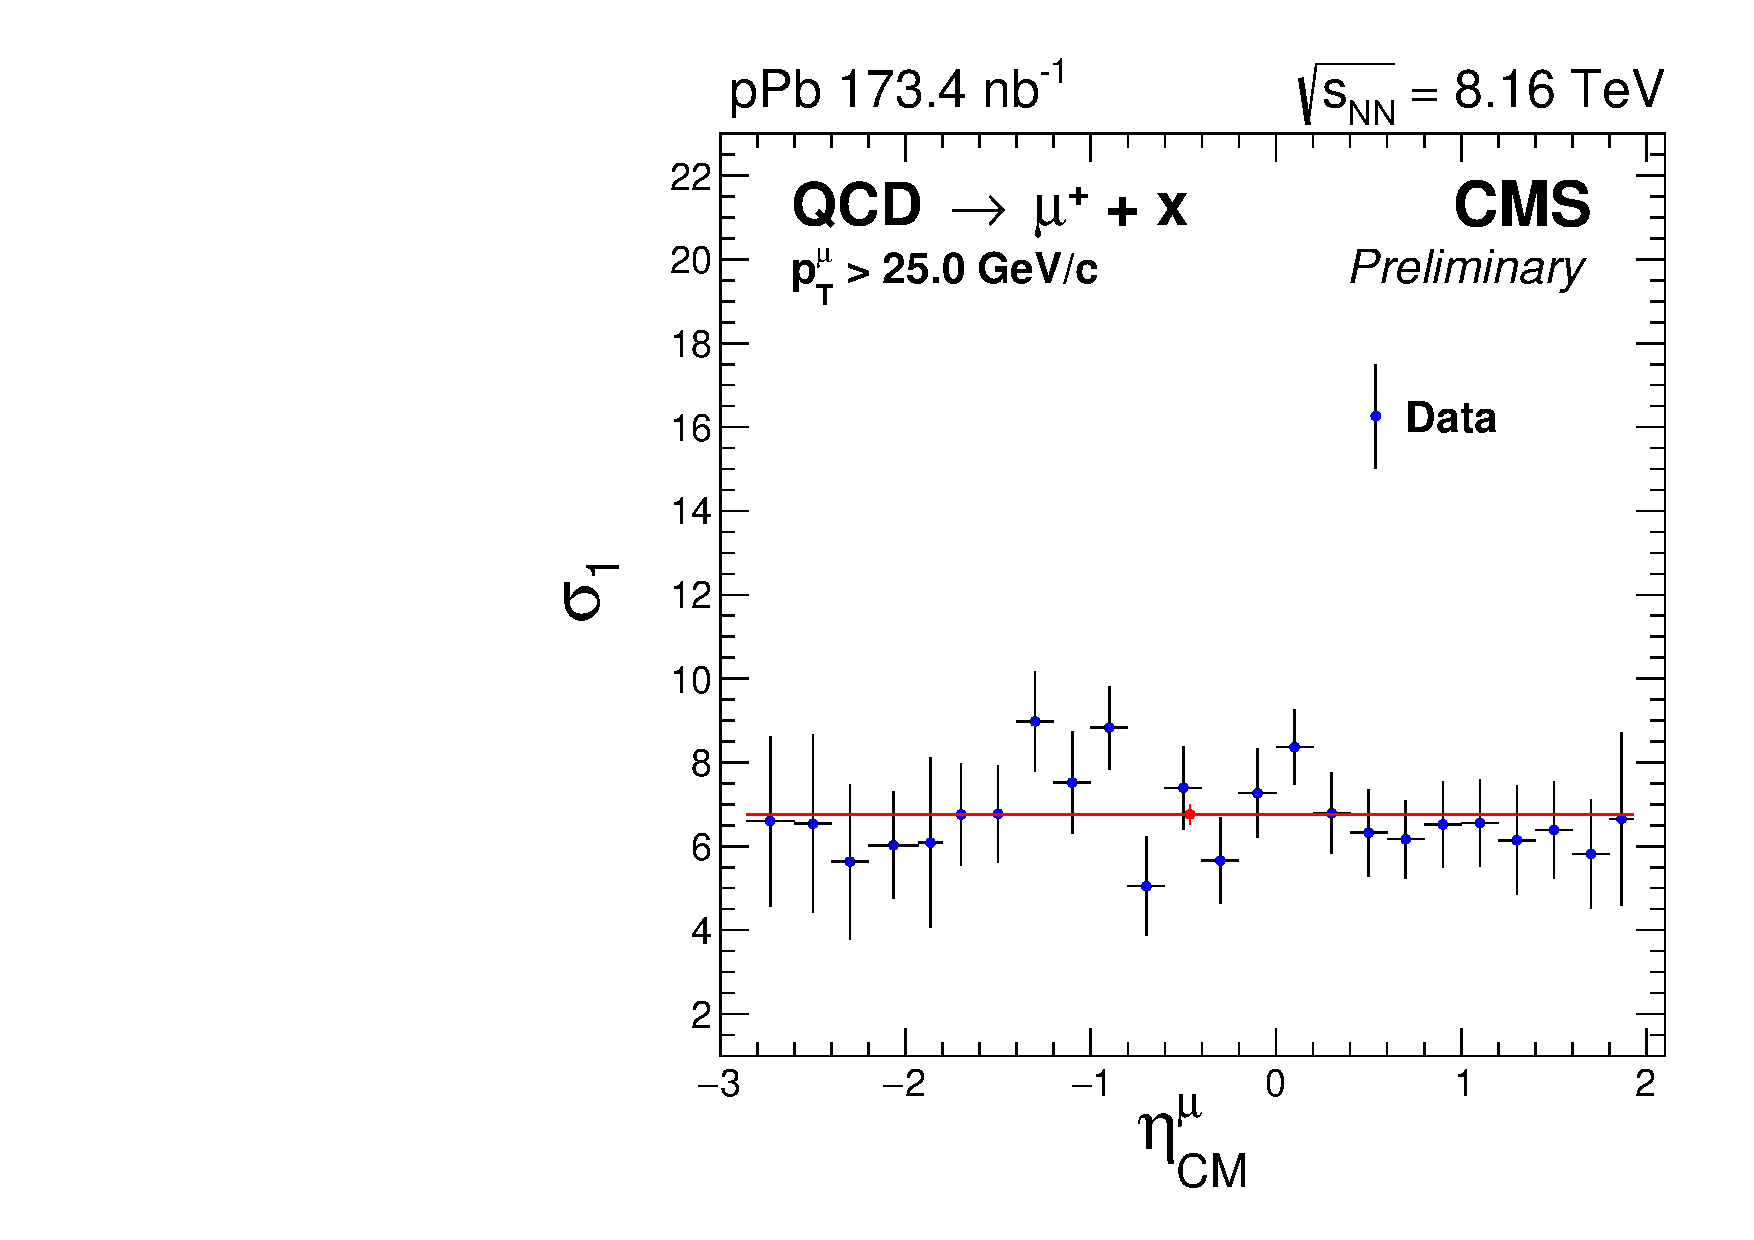
\includegraphics[width=0.32\textwidth]{Figures/WBoson/Analysis/SignalExtraction/QCD_Template/EXTRAPOLATION_ETA/exGraph_ETA_Sigma1_QCDToMuPl_PA.pdf}
  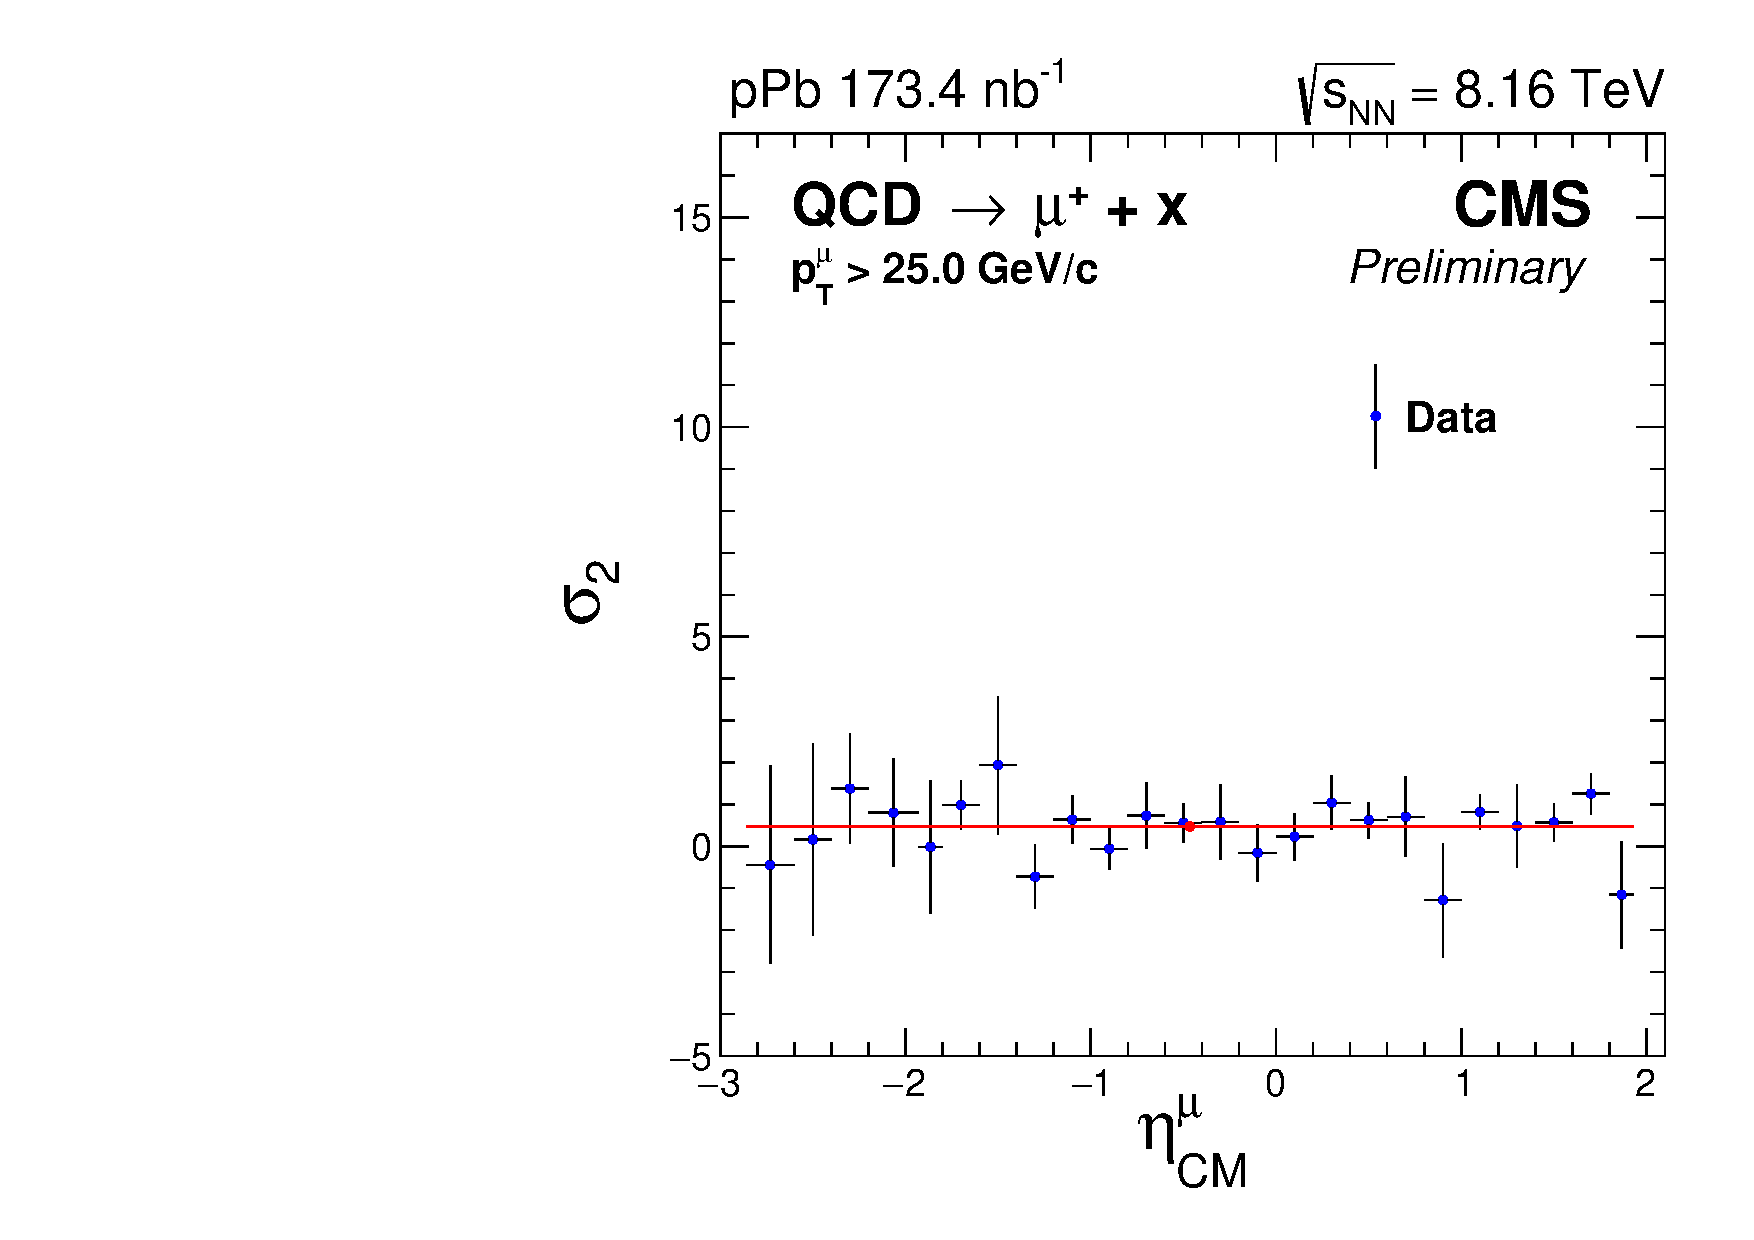
\includegraphics[width=0.32\textwidth]{Figures/WBoson/Analysis/SignalExtraction/QCD_Template/EXTRAPOLATION_ETA/exGraph_ETA_Sigma2_QCDToMuPl_PA.pdf}
 \caption{Muon $\etaMuCM$ dependence of $\sigma_{0}$ (left), $\sigma_{1}$ (middle) and $\sigma_{2}$ (right) parameters extrapolated to $\iso = 0.03$. The results are shown for negative (top) and positive (bottom) charged muons. The red line corresponds to the QCD jet parameter extrapolated in the \etaMuCM-inclusive range.}
 \label{fig:QCD_Extrapolation_Eta}
\end{figure}

It is observed that the $\sigma_{0}$, $\sigma_{1}$, and $\sigma_{2}$ parameters, extrapolated to low muon isolation, do not vary significantly with respect to \etaMuCM and are found to be consistent with the corresponding values obtained in the \etaMuCM-inclusive range. As a result, the extrapolated parameters derived in the \etaMuCM-inclusive range for $\mu^{+}$ and $\mu^{-}$, are used to fix the QCD jet background shape when fitting the signal.


\subsubsection{Modelling of the signal, \ttbar and electroweak backgrounds}\label{sec:WBoson_Analysis_SignalExtraction_EWKBackground}

The \ptmiss  distribution of the signal, as well as the \ttbar and electroweak background events, are estimated using the corresponding \POWHEG simulations mentioned in \sect{sec:WBoson_Analysis_Sample_MC}. The simulated events for each process are required to satisfy the signal selection criteria summarised in \sect{sec:WBoson_Analysis_Selection_WSelection}.

In order to improve the description of the data, several corrections are applied to the simulations. First, the simulated HF energy distribution is weighed as explained in \sect{sec:WBoson_Analysis_Corrections_EventActivityReweighing}. Then, the generated weak boson \pt distribution from the \WToMuNu, \WToTauNu, \DYToMuMu and \DYToTauTau simulations, is weighed as described in \sect{sec:WBoson_Analysis_Corrections_WeakBosonPTReweighing} And finally, the recoil of \WToMuNu, \WToTauNu and \DYToMuMu events is calibrated as detailed in \sect{sec:WBoson_Analysis_Corrections_RecoilCalib}, improving the agreement of the \ptmiss distribution between data and simulation.

Once the simulations have been corrected, the \ptmiss distribution of the signal, \ttbar background and electroweak background, are determined by building a template histogram of the simulated \ptmiss distribution (2~\GeVc bin width). These template histograms are then used in the fitting procedure describe in the next section.


\subsubsection{Fit model}\label{sec:WBoson_Analysis_SignalExtraction_FitModel}

The number of \WToMuNu signal events is obtained by performing an unbinned maximum-likelihood fit of the observed \ptmiss distribution in different muon \etaMuCM regions. The fits are done using a combination of template histograms and a functional form. The data analysis framework RooFit v3.60~\cite{RooFit} is used to make the fits.

The total fit model includes six contributions: the signal \WToMuNu template ($\euscr{T}_{\Wb}$), the electroweak background templates \DYToMuMu ($\euscr{T}_{\DYToMu}$), \WToTauNu ($\euscr{T}_{\WToTau}$) and \DYToTauTau ($\euscr{T}_{\DYToTau}$), the \ttbar background template ($\euscr{T}_{\ttbar}$), and the QCD jet background functional form ($\euscr{F}_{\QCD}$). The model used to fit the data is:

\begin{equation}
   N_{\Wb} \cdot \left( {\euscr{T}_{\Wb}} + {r_{\DYToMu} \cdot \euscr{T}_{\DYToMu}} + {r_{\WToTau} \cdot \euscr{T}_{\WToTau}} + {r_{\DYToTau} \cdot \euscr{T}_{\DYToTau}} + {r_{\ttbar} \cdot \euscr{T}_{\ttbar}} \right) + { N_{\QCD} \cdot \euscr{F}_{\QCD} }
 \label{eq:FitModel}
\end{equation}

where $N_{\Wb}$ and $N_{\QCD}$ are the normalisation factors of the \WToMuNu signal and QCD jet background component, $r_{\ttbar}$ represents the ratio of \ttbar background events over the number of signal events ($N_{\ttbar}\big/N_{\Wb}$), and 
$r_{\DYToMu}$, $r_{\DYToTau}$ and $r_{\WToTau}$ are the corresponding ratios for the \DYToMuMu, \DYToTauTau and \WToTauNu background processes, respectively.

The \ptmiss distributions of the signal, \ttbar background and electroweak background processes are defined based on template histograms extracted from simulations. Being very small and with a moderately discriminating shape, the  electroweak and \ttbar background components cannot be directly and independently fitted on data. Instead, we take advantage that their nuclear modification should be small and close to the one of the \Wb-boson signal. Thus, the ratios of \DYToMuMu, \DYToTauTau, \WToTauNu and \ttbar events over the number of \WToMuNu events, are fixed to the results from simulations after having normalised all the MC samples to the recorded integrated luminosity of data as detailed in \sect{sec:WBoson_Analysis_Sample_MC} and applied all analysis corrections and selection criteria.

The QCD jet background contribution is taken into account by means of a functional form depending on three parameters. For the fits to the \ptmiss distribution in the signal region, the $\sigma_{0}$ , $\sigma_{1}$ and $\sigma_{2}$ parameters are fixed to the extrapolated values mentioned in \tab{tab:QCD_Extrapolation}, and the normalisation is left free.

The \ptmiss distribution is fitted separately for \WToMuNuPl and \WToMuNuMi events. Only the signal ($N_{\Wb}$) and the QCD jet background ($N_{\QCD}$) normalisation factors are left free when fitting the signal region in data. The fits are done in the \etaMuCM-inclusive range and in bins of muon \etaMuCM. The results of the fits performed in the \etaMuCM-inclusive range are shown in \fig{fig:SignalFit} and those performed in the other muon \etaMuCM bins are presented in \app{app:WBoson_SignalExtraction_Fits}.

\begin{figure}[htb!]
 \centering
 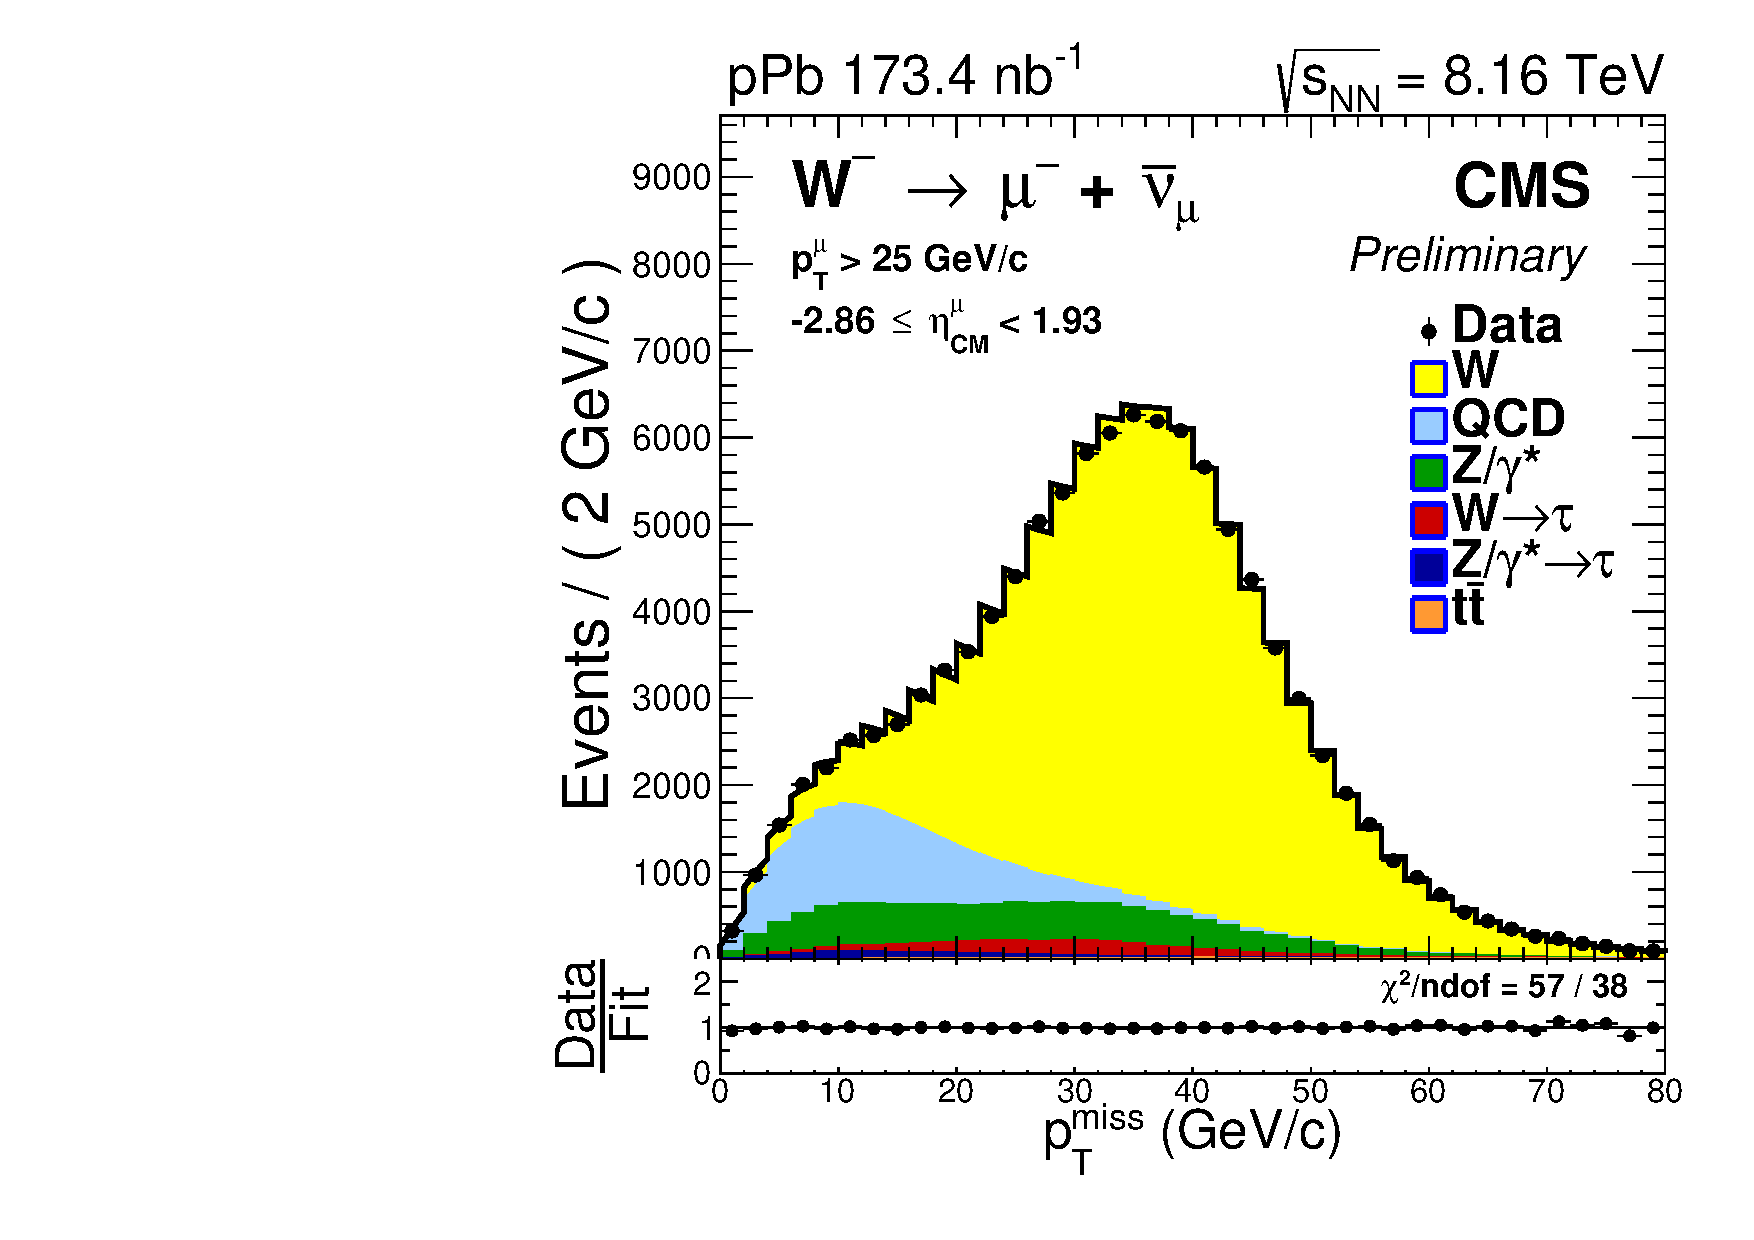
\includegraphics[width=0.45\textwidth]{Figures/WBoson/Analysis/SignalExtraction/Signal/LIN/PLOT_MET_DATA_WToMuMi_PA_Model_TEMP_WDYDYToTauWToTauTTbar_ModifiedRayleigh_QCD_MuEtaCM_-286_193_MuIso_0_15.pdf}
%%
 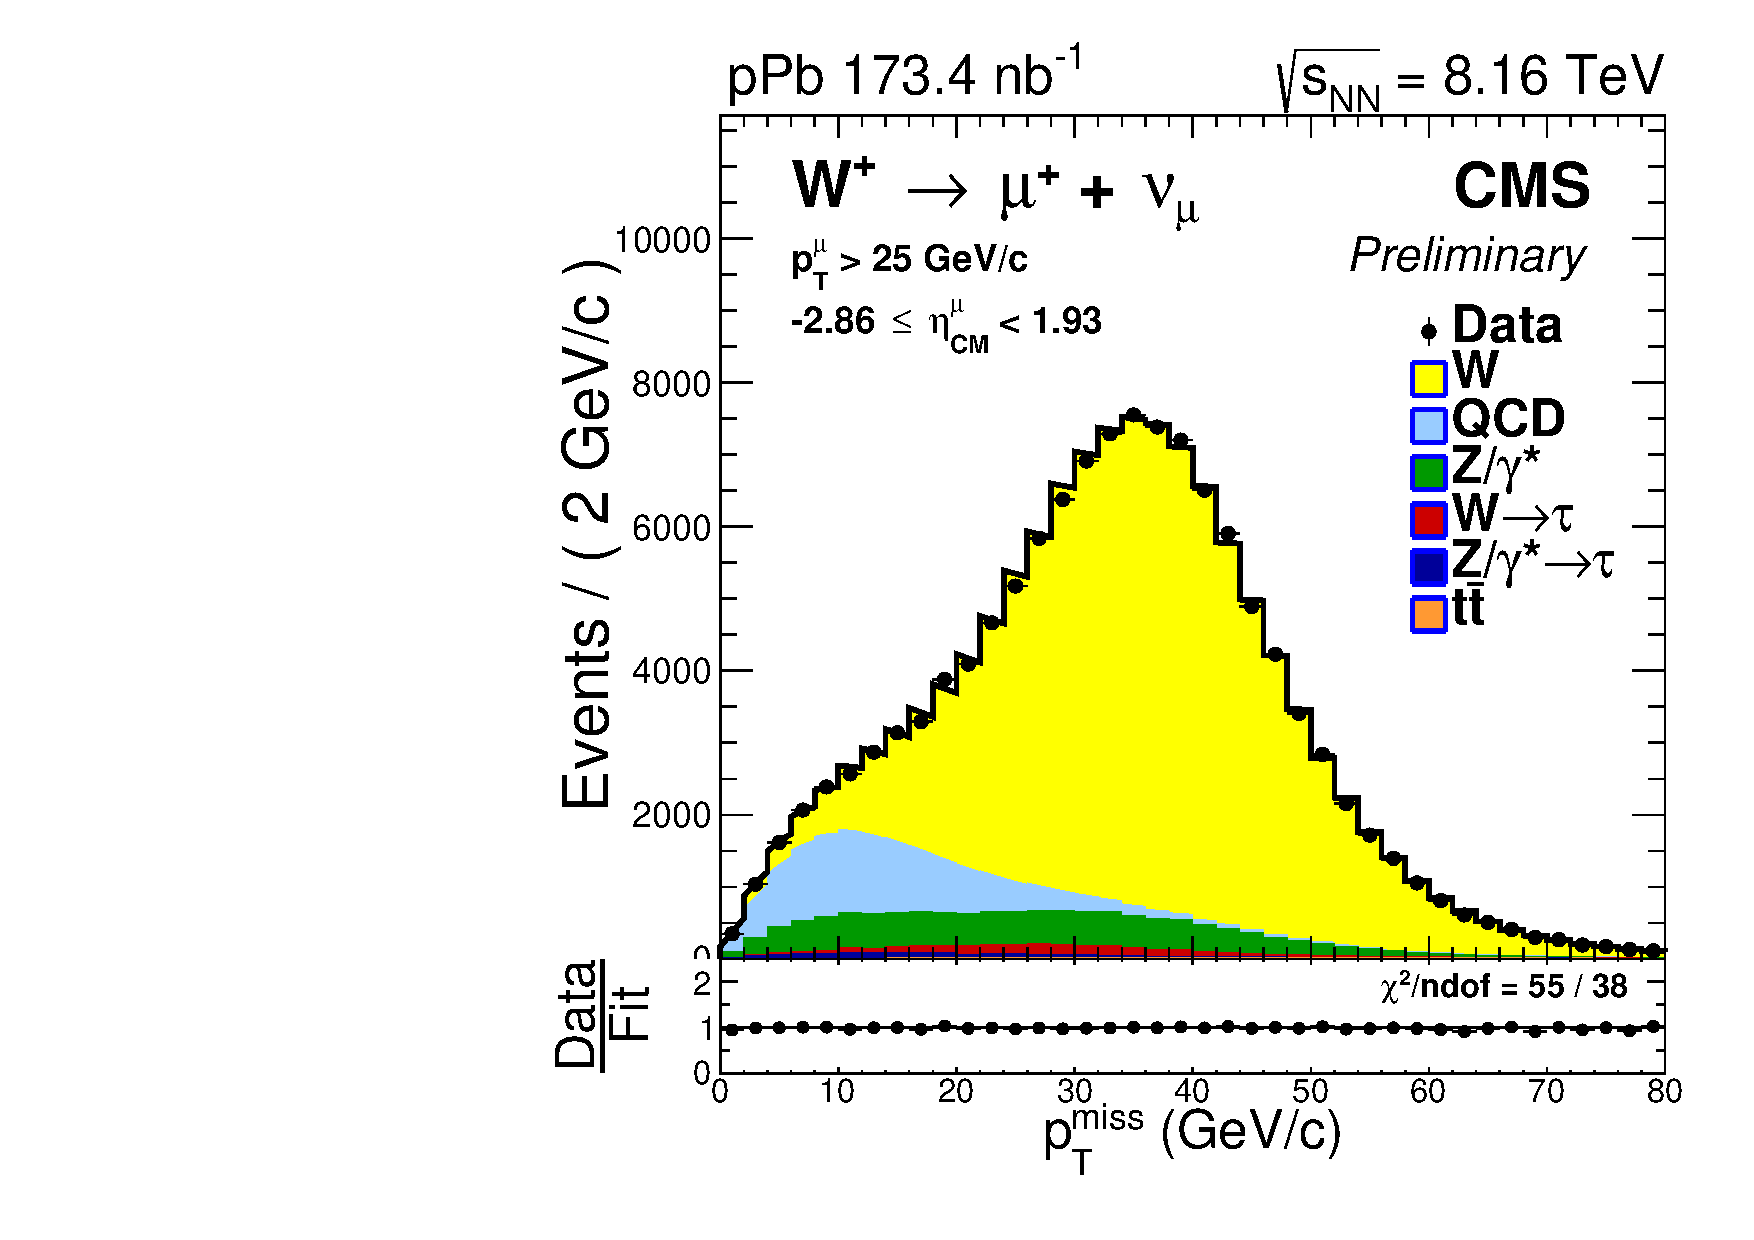
\includegraphics[width=0.45\textwidth]{Figures/WBoson/Analysis/SignalExtraction/Signal/LIN/PLOT_MET_DATA_WToMuPl_PA_Model_TEMP_WDYDYToTauWToTauTTbar_ModifiedRayleigh_QCD_MuEtaCM_-286_193_MuIso_0_15.pdf}
 \caption{The \ptmiss distribution for \WToMuNuMi (left) and  \WToMuNuPl (right) events within the \etaMuCM-inclusive range, shown in linear scale. Unbinned fits to the data (black points) are performed with six contributions, stacked from top to bottom: \WToMuNu (yellow), QCD jet (light blue), \DYToMuMu (green), \WToTauNu (red), \DYToTauTau (dark blue) and \ttbar (orange). The lower panel, on each figure, display the ratio of the measurements over the result of the fit. The Baker-Cousins~\cite{BakerCousins_Chi2} $\chi^{2}$ test value over the number of degrees of freedom is also shown.}
 \label{fig:SignalFit}
\end{figure}

\subsubsection{Extracted event yields}\label{sec:WBoson_Analysis_SignalExtraction_RawYields}

The results of the fits to the data in each of the different muon \etaCM bins are summarized in \tab{tab:RawYields_WToMuMi_PA} and \tab{tab:RawYields_WToMuPl_PA} for \WToMuNuMi and \WToMuNuPl events, respectively.

\begin{table}[htb!]
  \centering
  \resizebox{\textwidth}{!}{
  %\renewcommand{\arraystretch}{1.5}
  \begin{tabular}{|c|*7c|}
    \hline
    $\etaMuCM$ Range & Total & Signal & \DYToMuMu & \WToTauNu & \DYToTauTau & \ttbar & QCD\\
    \hline\hline
    $-$2.86 , $-$2.60 & 5210 & $4041 \pm 65$ & $560 \pm 9$ & $135 \pm 2$ & $45 \pm 1$ & $3.1 \pm 0.1$ & $427 \pm 40$\\
    \hline
    $-$2.60 , $-$2.40 & 4308 & $3395 \pm 60$ & $461 \pm 8$ & $102 \pm 2$ & $36 \pm 1$ & $4.0 \pm 0.1$ & $310 \pm 37$\\
    \hline
    $-$2.40 , $-$2.20 & 4273 & $3276 \pm 59$ & $449 \pm 8$ & $100 \pm 2$ & $36 \pm 1$ & $5.9 \pm 0.1$ & $407 \pm 38$\\
    \hline
    $-$2.20 , $-$1.93 & 6423 & $4920 \pm 74$ & $654 \pm 10$ & $156 \pm 2$ & $62 \pm 1$ & $12.9 \pm 0.2$ & $617 \pm 48$\\
    \hline
    $-$1.93 , $-$1.80 & 3140 & $2419 \pm 52$ & $303 \pm 6$ & $79 \pm 2$ & $28 \pm 1$ & $8.4 \pm 0.2$ & $302 \pm 34$\\
    \hline
    $-$1.80 , $-$1.60 & 4822 & $3672 \pm 64$ & $435 \pm 8$ & $117 \pm 2$ & $45 \pm 1$ & $15.2 \pm 0.3$ & $537 \pm 43$\\
    \hline
    $-$1.60 , $-$1.40 & 4727 & $3631 \pm 64$ & $390 \pm 7$ & $117 \pm 2$ & $39 \pm 1$ & $18.8 \pm 0.3$ & $533 \pm 43$\\
    \hline
    $-$1.40 , $-$1.20 & 4521 & $3590 \pm 64$ & $340 \pm 6$ & $109 \pm 2$ & $45 \pm 1$ & $21.6 \pm 0.4$ & $416 \pm 40$\\
    \hline
    $-$1.20 , $-$1.00 & 4626 & $3666 \pm 65$ & $306 \pm 5$ & $118 \pm 2$ & $48 \pm 1$ & $25.2 \pm 0.4$ & $463 \pm 42$\\
    \hline
    $-$1.00 , $-$0.80 & 4722 & $3762 \pm 66$ & $277 \pm 5$ & $119 \pm 2$ & $45 \pm 1$ & $32 \pm 1$ & $488 \pm 43$\\
    \hline
    $-$0.80 , $-$0.60 & 4198 & $3425 \pm 63$ & $238 \pm 4$ & $102 \pm 2$ & $46 \pm 1$ & $32 \pm 1$ & $355 \pm 39$\\
    \hline
    $-$0.60 , $-$0.40 & 4648 & $3738 \pm 66$ & $245 \pm 4$ & $119 \pm 2$ & $54 \pm 1$ & $35 \pm 1$ & $456 \pm 43$\\
    \hline
    $-$0.40 , $-$0.20 & 4344 & $3478 \pm 64$ & $226 \pm 4$ & $111 \pm 2$ & $50 \pm 1$ & $36 \pm 1$ & $443 \pm 41$\\
    \hline
    $-$0.20 , $+$0.00 & 4474 & $3510 \pm 65$ & $260 \pm 5$ & $113 \pm 2$ & $43 \pm 1$ & $39 \pm 1$ & $509 \pm 43$\\
    \hline
    $+$0.00 , $+$0.20 & 4643 & $3654 \pm 65$ & $309 \pm 6$ & $114 \pm 2$ & $47 \pm 1$ & $42 \pm 1$ & $477 \pm 43$\\
    \hline
    $+$0.20 , $+$0.40 & 4638 & $3533 \pm 64$ & $335 \pm 6$ & $111 \pm 2$ & $50 \pm 1$ & $42 \pm 1$ & $567 \pm 44$\\
    \hline
    $+$0.40 , $+$0.60 & 4718 & $3528 \pm 63$ & $390 \pm 7$ & $114 \pm 2$ & $46 \pm 1$ & $39 \pm 1$ & $601 \pm 44$\\
    \hline
    $+$0.60 , $+$0.80 & 4552 & $3375 \pm 62$ & $446 \pm 8$ & $103 \pm 2$ & $48 \pm 1$ & $37 \pm 1$ & $544 \pm 43$\\
    \hline
    $+$0.80 , $+$1.00 & 4637 & $3325 \pm 61$ & $489 \pm 9$ & $103 \pm 2$ & $43 \pm 1$ & $37 \pm 1$ & $640 \pm 44$\\
    \hline
    $+$1.00 , $+$1.20 & 4612 & $3265 \pm 60$ & $539 \pm 10$ & $105 \pm 2$ & $45 \pm 1$ & $29 \pm 1$ & $630 \pm 44$\\
    \hline
    $+$1.20 , $+$1.40 & 4053 & $2769 \pm 55$ & $517 \pm 10$ & $78 \pm 2$ & $38 \pm 1$ & $23.8 \pm 0.5$ & $627 \pm 42$\\
    \hline
    $+$1.40 , $+$1.60 & 4251 & $2917 \pm 56$ & $620 \pm 12$ & $96 \pm 2$ & $39 \pm 1$ & $21.5 \pm 0.4$ & $557 \pm 42$\\
    \hline
    $+$1.60 , $+$1.80 & 3844 & $2506 \pm 51$ & $611 \pm 12$ & $78 \pm 2$ & $35 \pm 1$ & $15.4 \pm 0.3$ & $599 \pm 41$\\
    \hline
    $+$1.80 , $+$1.93 & 2640 & $1719 \pm 42$ & $439 \pm 11$ & $54 \pm 1$ & $22 \pm 1$ & $9.6 \pm 0.2$ & $397 \pm 33$\\
    \hline
  \end{tabular}
  }
  \caption{Event yields of \WToMuNuMi and background processes, extracted from the fits to the \ptmiss distribution in each muon $\etaMuCM$ region. All analysis selection criteria are applied including the muon $p_{T} > 25$~GeV/c. All uncertainties shown are statistical only.}
  \label{tab:RawYields_WToMuMi_PA}
\end{table}


\begin{table}[htb!]
  \centering
  \resizebox{\textwidth}{!}{
  %\renewcommand{\arraystretch}{1.5}
  \begin{tabular}{|c|*7c|}
    \hline
    $\etaMuCM$ Range & Total & Signal & \DYToMuMu & \WToTauNu & \DYToTauTau & \ttbar & QCD\\
    \hline\hline
    $-$2.86 , $-$2.60 & 4465 & $3358 \pm 59$ & $583 \pm 10$ & $67 \pm 1$ & $44 \pm 1$ & $3.3 \pm 0.1$ & $409 \pm 38$\\
    \hline
    $-$2.60 , $-$2.40 & 4234 & $3247 \pm 58$ & $526 \pm 9$ & $65 \pm 1$ & $35 \pm 1$ & $4.2 \pm 0.1$ & $358 \pm 36$\\
    \hline
    $-$2.40 , $-$2.20 & 4377 & $3351 \pm 60$ & $500 \pm 9$ & $61 \pm 1$ & $36 \pm 1$ & $6.5 \pm 0.1$ & $423 \pm 38$\\
    \hline
    $-$2.20 , $-$1.93 & 6847 & $5257 \pm 76$ & $714 \pm 10$ & $101 \pm 1$ & $53 \pm 1$ & $14.3 \pm 0.2$ & $706 \pm 49$\\
    \hline
    $-$1.93 , $-$1.80 & 3592 & $2762 \pm 55$ & $335 \pm 7$ & $56 \pm 1$ & $29 \pm 1$ & $8.5 \pm 0.2$ & $400 \pm 36$\\
    \hline
    $-$1.80 , $-$1.60 & 5421 & $4299 \pm 69$ & $488 \pm 8$ & $94 \pm 2$ & $50 \pm 1$ & $16.0 \pm 0.3$ & $471 \pm 43$\\
    \hline
    $-$1.60 , $-$1.40 & 5343 & $4375 \pm 70$ & $446 \pm 7$ & $96 \pm 2$ & $45 \pm 1$ & $18.0 \pm 0.3$ & $364 \pm 42$\\
    \hline
    $-$1.40 , $-$1.20 & 5129 & $4182 \pm 69$ & $375 \pm 6$ & $98 \pm 2$ & $41 \pm 1$ & $23.4 \pm 0.4$ & $405 \pm 43$\\
    \hline
    $-$1.20 , $-$1.00 & 5382 & $4465 \pm 72$ & $339 \pm 5$ & $100 \pm 2$ & $53 \pm 1$ & $28.3 \pm 0.5$ & $395 \pm 43$\\
    \hline
    $-$1.00 , $-$0.80 & 5467 & $4485 \pm 73$ & $306 \pm 5$ & $100 \pm 2$ & $50 \pm 1$ & $32 \pm 1$ & $491 \pm 45$\\
    \hline
    $-$0.80 , $-$0.60 & 4738 & $3960 \pm 68$ & $244 \pm 4$ & $89 \pm 2$ & $42 \pm 1$ & $29 \pm 1$ & $373 \pm 41$\\
    \hline
    $-$0.60 , $-$0.40 & 5349 & $4435 \pm 73$ & $255 \pm 4$ & $99 \pm 2$ & $49 \pm 1$ & $38 \pm 1$ & $473 \pm 45$\\
    \hline
    $-$0.40 , $-$0.20 & 5027 & $4146 \pm 70$ & $238 \pm 4$ & $88 \pm 1$ & $46 \pm 1$ & $37 \pm 1$ & $468 \pm 43$\\
    \hline
    $-$0.20 , $+$0.00 & 5161 & $4269 \pm 71$ & $268 \pm 4$ & $99 \pm 2$ & $45 \pm 1$ & $39 \pm 1$ & $439 \pm 43$\\
    \hline
    $+$0.00 , $+$0.20 & 5473 & $4352 \pm 72$ & $308 \pm 5$ & $100 \pm 2$ & $52 \pm 1$ & $39 \pm 1$ & $621 \pm 47$\\
    \hline
    $+$0.20 , $+$0.40 & 5175 & $4179 \pm 70$ & $337 \pm 6$ & $99 \pm 2$ & $48 \pm 1$ & $37 \pm 1$ & $475 \pm 44$\\
    \hline
    $+$0.40 , $+$0.60 & 5482 & $4334 \pm 71$ & $399 \pm 7$ & $93 \pm 2$ & $43 \pm 1$ & $36 \pm 1$ & $576 \pm 46$\\
    \hline
    $+$0.60 , $+$0.80 & 5722 & $4469 \pm 72$ & $469 \pm 8$ & $99 \pm 2$ & $51 \pm 1$ & $38 \pm 1$ & $595 \pm 47$\\
    \hline
    $+$0.80 , $+$1.00 & 6061 & $4652 \pm 72$ & $561 \pm 9$ & $99 \pm 2$ & $48 \pm 1$ & $37 \pm 1$ & $664 \pm 48$\\
    \hline
    $+$1.00 , $+$1.20 & 5814 & $4404 \pm 70$ & $595 \pm 9$ & $102 \pm 2$ & $41 \pm 1$ & $33 \pm 1$ & $639 \pm 47$\\
    \hline
    $+$1.20 , $+$1.40 & 5365 & $4050 \pm 67$ & $570 \pm 9$ & $87 \pm 1$ & $35 \pm 1$ & $23.9 \pm 0.4$ & $596 \pm 45$\\
    \hline
    $+$1.40 , $+$1.60 & 5768 & $4308 \pm 68$ & $674 \pm 11$ & $92 \pm 1$ & $39 \pm 1$ & $21.5 \pm 0.3$ & $633 \pm 46$\\
    \hline
    $+$1.60 , $+$1.80 & 5320 & $3969 \pm 65$ & $662 \pm 11$ & $81 \pm 1$ & $34 \pm 1$ & $16.1 \pm 0.3$ & $557 \pm 44$\\
    \hline
    $+$1.80 , $+$1.93 & 3600 & $2654 \pm 53$ & $450 \pm 9$ & $63 \pm 1$ & $19.8 \pm 0.4$ & $9.3 \pm 0.2$ & $404 \pm 36$\\
    \hline
  \end{tabular}
  }
  \caption{Event yields of \WToMuNuPl and background processes, extracted from the fits to the \ptmiss distribution in each muon $\etaMuCM$ region. All analysis selection criteria are applied including the muon $p_{T} > 25$~GeV/c. All uncertainties shown are statistical only.}
  \label{tab:RawYields_WToMuPl_PA}
\end{table}




\subsubsection{Corrected event yields}\label{sec:WBoson_Analysis_SignalExtraction_CorrectedYields}

The signal event yields extracted from the fits are corrected by taking into account the efficiency of the detector, according to:

\begin{equation}
 N^{\pm}_{\mu}\left(\etaMuCM\right) = \frac{N^{\pm}_{\mu,\text{raw}}\left(\etaMuCM\right)}{\epsilon^{\pm}_{\corr}\left(\etaMuCM\right)}
 \label{eq:CorrectedYield}
\end{equation}

where $N_{\mu,\text{raw}}$ is the number of signal events extracted from the fits, $N_{\mu}$ is the number of signal events after correcting for efficiency and $\epsilon_{\corr}^{\pm}$ is the signal efficiency corrected with the TnP corrections. The statistical uncertainty of the corrected signal yields are computed based on error propagation with:

\begin{equation}
 \delta{N^{\pm}_{\mu}} = \frac{\delta{N^{\pm}_{\mu,\text{raw}}}\left(\etaMuCM\right)}{\epsilon^{\pm}_{\corr}\left(\etaMuCM\right)}
\label{eq:CorrectedYieldStatError}
\end{equation}

where $\delta{N^{\pm}_{\mu,\text{raw}}}$ is the uncertainty of the signal event yield determined from the fits to the data. The results of the corrected signal event yields for each muon \etaMuCM range are summarized in \tab{tab:CorrYields_WToMuMi_PA} and \tab{tab:CorrYields_WToMuPl_PA} for \WToMuNuMi and \WToMuNuPl events, accordingly.

\begin{table}[htb!]
  \centering
  %\renewcommand{\arraystretch}{1.5}
  \begin{tabular}{|c|*3c|}
    \hline
    $\etaMuCM$ Range & Extracted yield & Efficiency ($\%$) & Corrected yield\\
    \hline\hline
    $-$2.86 , $-$2.60 & $4041 \pm 65$ & $84.7 \pm 0.2$ & $4773 \pm 77$\\
    \hline
    $-$2.60 , $-$2.40 & $3395 \pm 60$ & $87.3 \pm 0.2$ & $3891 \pm 69$\\
    \hline
    $-$2.40 , $-$2.20 & $3276 \pm 59$ & $83.8 \pm 0.2$ & $3907 \pm 71$\\
    \hline
    $-$2.20 , $-$1.93 & $4920 \pm 74$ & $87.6 \pm 0.2$ & $5619 \pm 84$\\
    \hline
    $-$1.93 , $-$1.80 & $2419 \pm 52$ & $92.1 \pm 0.2$ & $2627 \pm 56$\\
    \hline
    $-$1.80 , $-$1.60 & $3672 \pm 64$ & $92.0 \pm 0.1$ & $3990 \pm 70$\\
    \hline
    $-$1.60 , $-$1.40 & $3631 \pm 64$ & $88.7 \pm 0.2$ & $4093 \pm 72$\\
    \hline
    $-$1.40 , $-$1.20 & $3590 \pm 64$ & $85.5 \pm 0.2$ & $4200 \pm 75$\\
    \hline
    $-$1.20 , $-$1.00 & $3666 \pm 65$ & $89.4 \pm 0.2$ & $4102 \pm 73$\\
    \hline
    $-$1.00 , $-$0.80 & $3762 \pm 66$ & $89.7 \pm 0.2$ & $4195 \pm 74$\\
    \hline
    $-$0.80 , $-$0.60 & $3425 \pm 63$ & $81.1 \pm 0.2$ & $4222 \pm 78$\\
    \hline
    $-$0.60 , $-$0.40 & $3738 \pm 66$ & $88.7 \pm 0.2$ & $4216 \pm 75$\\
    \hline
    $-$0.40 , $-$0.20 & $3478 \pm 64$ & $83.8 \pm 0.2$ & $4148 \pm 76$\\
    \hline
    $-$0.20 , $+$0.00 & $3510 \pm 65$ & $87.5 \pm 0.2$ & $4012 \pm 74$\\
    \hline
    $+$0.00 , $+$0.20 & $3654 \pm 65$ & $89.3 \pm 0.2$ & $4091 \pm 73$\\
    \hline
    $+$0.20 , $+$0.40 & $3533 \pm 64$ & $85.8 \pm 0.2$ & $4116 \pm 74$\\
    \hline
    $+$0.40 , $+$0.60 & $3528 \pm 63$ & $88.2 \pm 0.2$ & $4000 \pm 72$\\
    \hline
    $+$0.60 , $+$0.80 & $3375 \pm 62$ & $90.5 \pm 0.2$ & $3729 \pm 68$\\
    \hline
    $+$0.80 , $+$1.00 & $3325 \pm 61$ & $92.1 \pm 0.2$ & $3610 \pm 66$\\
    \hline
    $+$1.00 , $+$1.20 & $3265 \pm 60$ & $88.2 \pm 0.2$ & $3704 \pm 68$\\
    \hline
    $+$1.20 , $+$1.40 & $2769 \pm 55$ & $83.5 \pm 0.2$ & $3318 \pm 65$\\
    \hline
    $+$1.40 , $+$1.60 & $2917 \pm 56$ & $90.6 \pm 0.2$ & $3219 \pm 61$\\
    \hline
    $+$1.60 , $+$1.80 & $2506 \pm 51$ & $83.4 \pm 0.2$ & $3005 \pm 61$\\
    \hline
    $+$1.80 , $+$1.93 & $1719 \pm 42$ & $86.4 \pm 0.3$ & $1990 \pm 48$\\
    \hline
  \end{tabular}
  \caption{Corrected event yields of \WToMuNuMi, given for each muon $\etaMuCM$ bin. All analysis selection criteria are applied including the muon $p_{T} > 25$~GeV/c. The muon efficiency has been corrected by applying the tag-and-probe corrections, HF energy weights and vector boson \pt weights, event by event. All uncertainties shown are statistical only.}
  \label{tab:CorrYields_WToMuMi_PA}
\end{table}


\begin{table}[htb!]
  \centering
  %\renewcommand{\arraystretch}{1.5}
  \begin{tabular}{|c|*3c|}
    \hline
    $\etaMuCM$ Range & Extracted yield & Efficiency ($\%$) & Corrected yield\\
    \hline\hline
    $-$2.86 , $-$2.60 & $3358 \pm 59$ & $84.3 \pm 0.2$ & $3982 \pm 70$\\
    \hline
    $-$2.60 , $-$2.40 & $3247 \pm 58$ & $87.3 \pm 0.2$ & $3721 \pm 66$\\
    \hline
    $-$2.40 , $-$2.20 & $3351 \pm 60$ & $83.8 \pm 0.2$ & $3997 \pm 71$\\
    \hline
    $-$2.20 , $-$1.93 & $5257 \pm 76$ & $86.8 \pm 0.2$ & $6055 \pm 87$\\
    \hline
    $-$1.93 , $-$1.80 & $2762 \pm 55$ & $92.0 \pm 0.2$ & $3001 \pm 60$\\
    \hline
    $-$1.80 , $-$1.60 & $4299 \pm 69$ & $91.9 \pm 0.1$ & $4679 \pm 75$\\
    \hline
    $-$1.60 , $-$1.40 & $4375 \pm 70$ & $88.7 \pm 0.2$ & $4931 \pm 79$\\
    \hline
    $-$1.40 , $-$1.20 & $4182 \pm 69$ & $84.7 \pm 0.2$ & $4940 \pm 82$\\
    \hline
    $-$1.20 , $-$1.00 & $4465 \pm 72$ & $88.4 \pm 0.2$ & $5049 \pm 81$\\
    \hline
    $-$1.00 , $-$0.80 & $4485 \pm 73$ & $89.2 \pm 0.2$ & $5029 \pm 82$\\
    \hline
    $-$0.80 , $-$0.60 & $3960 \pm 68$ & $80.7 \pm 0.2$ & $4908 \pm 85$\\
    \hline
    $-$0.60 , $-$0.40 & $4435 \pm 73$ & $88.5 \pm 0.2$ & $5015 \pm 83$\\
    \hline
    $-$0.40 , $-$0.20 & $4146 \pm 70$ & $83.0 \pm 0.2$ & $4996 \pm 85$\\
    \hline
    $-$0.20 , $+$0.00 & $4269 \pm 71$ & $87.2 \pm 0.2$ & $4897 \pm 81$\\
    \hline
    $+$0.00 , $+$0.20 & $4352 \pm 72$ & $89.2 \pm 0.2$ & $4881 \pm 81$\\
    \hline
    $+$0.20 , $+$0.40 & $4179 \pm 70$ & $85.0 \pm 0.2$ & $4915 \pm 82$\\
    \hline
    $+$0.40 , $+$0.60 & $4334 \pm 71$ & $88.3 \pm 0.2$ & $4908 \pm 81$\\
    \hline
    $+$0.60 , $+$0.80 & $4469 \pm 72$ & $90.4 \pm 0.2$ & $4944 \pm 79$\\
    \hline
    $+$0.80 , $+$1.00 & $4652 \pm 72$ & $91.6 \pm 0.2$ & $5081 \pm 79$\\
    \hline
    $+$1.00 , $+$1.20 & $4404 \pm 70$ & $87.8 \pm 0.2$ & $5016 \pm 80$\\
    \hline
    $+$1.20 , $+$1.40 & $4050 \pm 67$ & $83.2 \pm 0.2$ & $4867 \pm 80$\\
    \hline
    $+$1.40 , $+$1.60 & $4308 \pm 68$ & $90.3 \pm 0.2$ & $4773 \pm 76$\\
    \hline
    $+$1.60 , $+$1.80 & $3969 \pm 65$ & $83.1 \pm 0.2$ & $4776 \pm 78$\\
    \hline
    $+$1.80 , $+$1.93 & $2654 \pm 53$ & $86.9 \pm 0.2$ & $3054 \pm 61$\\
    \hline
  \end{tabular}
  \caption{Corrected event yields of \WToMuNuPl, given for each muon $\etaMuCM$. All analysis selection criteria are applied including the muon $p_{T} > 25$~GeV/c. The muon efficiency has been corrected by applying the tag-and-probe corrections, HF energy weights and vector boson \pt weights, event by event. All uncertainties shown are statistical only.}
  \label{tab:CorrYields_WToMuPl_PA}
\end{table}






% END OF SUBSECTION